\documentclass[twocolumn]{article} % Two-column document

% Packages for formatting
\usepackage[utf8]{inputenc}
\usepackage{amsmath}
\usepackage{geometry}
\usepackage{graphicx}
\usepackage{lipsum} % for filler text
\usepackage{authblk} % For author affiliations
\usepackage[utf8]{inputenc}
\usepackage{hyperref}

\usepackage{textcomp}
\usepackage{charter}
\usepackage{framed}

\usepackage{verbatim}
\usepackage{fancyvrb}
\usepackage{booktabs}

\usepackage{caption}  % For custom captions
\usepackage{subcaption} % For subfigures/subtables
\usepackage{array}    % For array and tabular options

\usepackage{float}
\usepackage{ulem}
\usepackage{pifont}



\hypersetup{
    colorlinks=true,
    linkcolor=blue,
    filecolor=magenta,      
    urlcolor=cyan,
    pdftitle={Overleaf Example},
    pdfpagemode=FullScreen,
}

% Page setup
\geometry{a4paper, margin=0.5in}

% Title and Author formatting
\makeatletter
\renewcommand{\maketitle}{
    \bgroup\setlength{\parindent}{0pt}
        \begin{flushleft}
        \textbf{\@title\newline}
        
        \@author
        \end{flushleft}
    \egroup
}
\makeatother

% Title
\title{\fontsize{40}{1}\usefont{T1}{cmr}{b}{n} Modeling Student Performance: Using Multiple Linear Regression to Predict Exam Scores \vspace{0.05cm}}

% Authors
\author[1]{Victoria Blante}
\author[2]{Chelyah Miller}
\author[3]{Xiaonan Song}
\author[4]{Emma Juan Salazar}

% Author affiliations
\affil[*]{University of San Francisco, Master of Science in Data Science\newline}

% Email
\affil[1]{vbblante@dons.usfca.edu}
\affil[2]{cmiller9@dons.usfca.edu}
\affil[3]{xsong20@dons.usfca.edu}
\affil[4]{ejuansalazar@dons.usfca.edu}

\renewcommand\Authands{ and }

\date{\today} % You can manually enter a date if needed

% Define path where images are stored
\graphicspath{ {./images/} }

% Define abstract format
\renewenvironment{abstract}
 {\small
  \begin{center}
  \bfseries \abstractname\vspace{-.5em}\vspace{0pt}
  \end{center}
  \list{}{%
    \setlength{\leftmargin}{10mm}% <---------- Change margin here
    \setlength{\rightmargin}{\leftmargin}%
  }%
  \item\relax}
 {\endlist}

% Begin the document
\begin{document}

% Print out title and abstract
\twocolumn[
\begin{@twocolumnfalse}

\maketitle

\begin{abstract}
\textit{
  This study explores the factors influencing student performance by applying multiple linear regression models to predict exam scores. Using a dataset of 6,378 students, we analyzed both numerical variables, such as hours studied, attendance, and previous scores, as well as categorical variables, including motivation level, access to resources, and family income. Due to clustering of exam scores around 65\%, we split the data into two groups: high-performing students (scores $\geq 80$) and average-performing students (scores $< 80$). The average-performing model achieved an adjusted $R^2$ of 0.898, indicating strong predictive power, while the high-performing model had an adjusted $R^2$ of 0.602 due to limited data. Our results highlight that study habits, attendance, prior performance, and socioeconomic factors significantly impact academic outcomes.
    \bigskip}
\end{abstract}

% Keywords
\textbf{Keywords:} Multiple Linear Regression, Modeling

\bigskip
\bigskip
\bigskip

\end{@twocolumnfalse}
]

% INTRODUCTION
\section{Introduction}
\subsection*{Our Dataset}

The \href{https://www.kaggle.com/datasets/lainguyn123/student-performance-factors}{Student Performance Factors} dataset contains 20 variables with information about 6607 students.

This dataset includes information about the different habits a student has, like hours studied, attendance, extracurricular activities, physical activity, or the amount of hours they sleep

We also have information about the student's environment including Parental Involvement, peer influence, school type, or teacher quality.

Moreover, we have information about the student themselves, like their gender, whether or not they have a learning disability, their motivation level, how many tutoring sessions they attend, their previous scores and their exam scores.

Additionally, it covers socioeconomic and background data such as family income, access to resources, internet access, and parental education level.

\subsection*{Purpose and Applications}\label{purpose-and-applications}

Our aim is to identify a response variable that will be indicative of student performance, and build a regression model to identify significant factors affecting student academic performance. This analysis' potential applications include:

\begin{itemize}
\item
    Supporting educational decision-making
\item
    Assisting in policy formulation
\item
    Optimizing the allocation of educational resources
\end{itemize}

Ultimately, the goal is to better understand and improve the key factors
influencing student success, thereby enabling educators and policymakers
to provide more targeted support.

\subsection*{Variable Descriptions}\label{variable-descriptions}

\begin{itemize}
\item
  \texttt{Hours\_Studied}: Daily study hours.
\item
  \texttt{Attendance}: Attendance rate (percentage).
\item
  \texttt{Parental\_Involvement}: Parent involvement (Low, Medium, High).
\item
  \texttt{Access\_to\_Resources}: Resource accessibility (Low, Medium, High).
\item
  \texttt{Extracurricular\_Activities}: Participation in extracurricular
  activities.
\item
  \texttt{Sleep\_Hours}: Daily sleep hours.
\item
  \texttt{Previous\_Scores}: Prior exam scores.
\item
  \texttt{Motivation\_Level}: Motivation level (Low, Medium, High).
\item
  \texttt{Internet\_Access}: Internet access.
\item
  \texttt{Tutoring\_Sessions}: Number of tutoring sessions.
\item
  \texttt{Family\_Income}: Family income level (Low, Medium, High).
\item
  \texttt{Teacher\_Quality}: Teacher quality (Low, Medium, High).
\item
  \texttt{School\_Type}: School type (Public or Private).
\item
  \texttt{Peer\_Influence}: Peer influence (Positive, Neutral,
  Negative).
\item
  \texttt{Physical\_Activity}: Weekly physical activity hours.
\item
  \texttt{Learning\_Disabilities}: Presence of learning disabilities.
\item
  \texttt{Parental\_Education\_Level}: Parents' education level (High School, College, Postgraduate).
\item
  \texttt{Distance\_from\_Home}: Distance from home to school (Near, Moderate, Far).
\item
  \texttt{Gender}: Student gender (Male or Female).
\item
  \texttt{Exam\_Score}: Academic performance indicator (exam score).
\end{itemize}

% METHODS
\section{Methods}
We used various methods to perform our analysis, from EDA all the way to Model Evaluation. Here's a detailed description of the methods and tools we used.

\begin{itemize}
\item
  \textbf{Exploratory Data Analysis}:
  Initial analysis includes
  correlation calculations to understand the relationships between
  predictors and exam scores.
\item
  \textbf{Multiple Linear Regression}:
  Regression models are built using
  significant predictors such as attendance, hours studied, and previous
  scores. The model is validated using metrics like adjusted R-squared,
  p-values, and F-statistics.
\item
  \textbf{ANOVA (Types I, II, and III)}:
  Variance analysis is conducted
  to understand the contribution of each predictor to the total variance
  in exam scores.
\item
  \textbf{Model Evaluation}:
  The model's prediction capability is
  visualized through plots of actual vs.~predicted exam scores,
  residuals distribution, and summary statistics.
\end{itemize}

% RESEARCH QUESTIONS

\section{Exploratory Data Analysis}
The Student Performance Factors dataset has 20 variables and 6607 observations. We have 7 numerical variables, including hours studied, attendance, sleep hours, previous scores, tutoring sessions, physical activity and exam score. The other 13 variables are categorical, having either 2 or 3 categories each.
This gives us enough room to be able to perform a comprehensive Multiple Linear Regression Analysis.

Before delving into our dataset, we checked for missing data. Only three of our columns had missing values (\texttt{Teacher\_Quality}, \texttt{Parental\_Education\_Level} and \texttt{Distance\_from\_Home}). Each of these columns has less than 2\% of missingness. Seeing as we have a substantial number of observations, we decided to go ahead and drop all observations with missing data (229 rows).

Our dataset size after this was of 20 variables and 6378 records.

\subsection*{Categorical variables}

Our first approach to get a sense of our categorical data was to plot the frequency for each category. See these plots in Supplementary Figure \ref{1:barplots}.

These plots allowed us to see that some categorical variables had similar shaped barplots. To optimize our categorical variables we drew up confusion tables to ascertain whether or not to collapse some of these variables.

We made confusion tables to check \texttt{Parental\_Involvment} against \texttt{Access\_to\_Resources} (Supplementary Table \ref{tab:confusion1}), \texttt{Family\_Income} against \texttt{Peer\_Influence} (Supplementary Table \ref{tab:confusion2}), \texttt{Distance\_from\_Home} against \texttt{Motivation\_Level} (Supplementary Table \ref{tab:confusion3}) and \texttt{Distance\_from\_Home} against \texttt{Motivation\_Level} (Supplementary Table \ref{tab:confusion3})

These confusion tables aided us to make the decision to drop the variables \texttt{Distance\_from\_Home}, \texttt{Peer\_Influence} and \texttt{Parental\_Involvment}.

\subsection*{Numerical Variables}

As a first approach, for the numerical variables, we drew boxplots to check their distributions and whether or not we see any outliers (Supplementary Figure \ref{2:boxplots})

From these boxplots, we saw that for tutoring sessions we have a few outliers in the upper levels but most of the observations are clustered around 1/2 tutoring sessions. We can also see that for exam score, most of the students in our dataset have scores clustered around 65 out of 100, and we have a few high performing students. We'll have to keep these in mind when picking our response variable.

Next, we decided to make a pairwise plot (Supplementary Figure \ref{3:pairwise}), a very powerful tool to try and get a first glance at which numerical variables seem to have linear relationships between one another.

A lot of our variables numerical variables are discrete and therefore the scatterplots show very distinct levels. Aside from these, there's a few scatterplots where we can see some sort of linearity between two variables. We can very clearly see that all of these plots include the variable \texttt{Exam\_Score}.

Looking at the histogram for Exam Score inside of the pairwise plot, we can very clearly see how it's clustered around lower scores, therefore indicating we don't have a normal distribution for these. We'll have to keep this fact in mind when analyzing this variable.

Lastly, we made a correlation heatmap (Figure \ref{4:corr-heatmap}), to assess how are variables are correlated between one another and get a first glance towards multicollinearity.

\begin{figure*}[h]
  \centering
  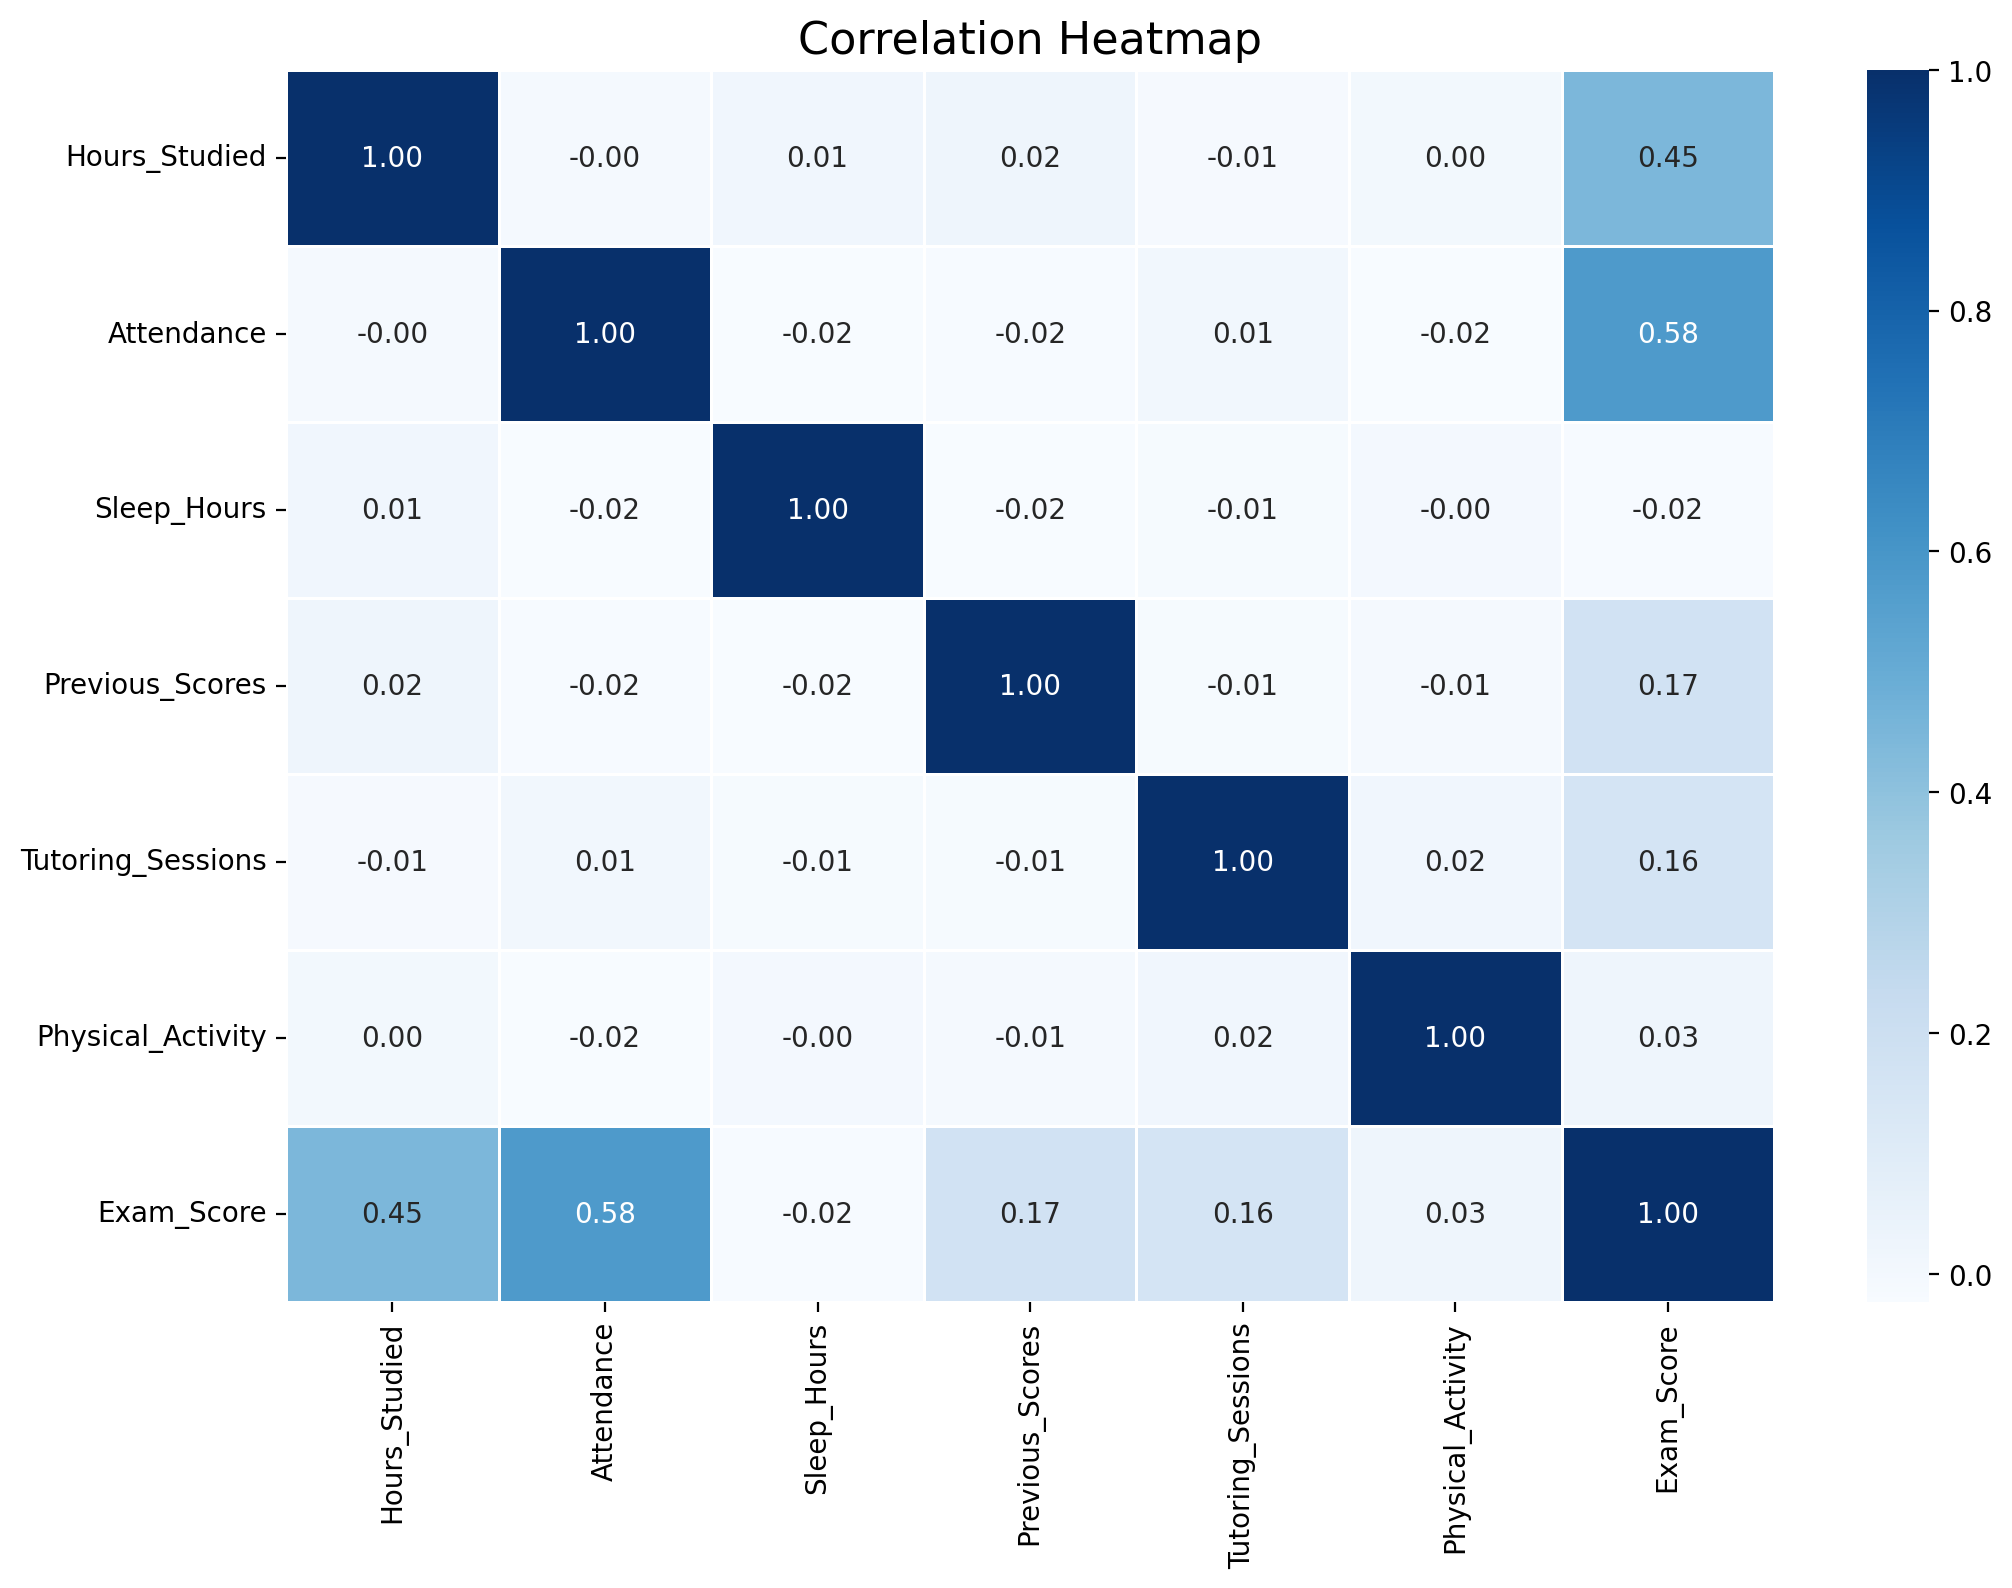
\includegraphics[width=0.9\linewidth]{4-correlation-heatmap.png}
  \caption{Heatmap depicting the correlation between our numerical variables.}
  \label{4:corr-heatmap}
\end{figure*}

We can see how the variable that has the most correlation to other variables is Exam Score, and how there's next to no correlation among the other variables. This indicates that picking Exam Score as our response variable seems a prudent choice, as it looks to be correlated to our other variables and also makes it so we have lower chances of having multicollinearity.

\newpage
\section{Hypotheses}

\subsection*{Hypothesising based on our EDA}
Since we were able to see some linear relationship between a few of our numerical variables and \texttt{Exam\_Score}, we have decided to pick this variable as our response variable.

The correlation heatmap also supports our choice of response variable, where we can see correlation between exam scores and the rest of the variables.

In the context of our problem, modeling student performance, we think choosing exam scores as our response variable is a good way to ascertain how students perform, and which factors influence the way they score in tests.

We have initially seen linearity in the scatterplots between exam score and hours studied, attendance, previous scores and tutoring sessions. We'll try to assess whether or not these numerical variables are statistically significant when predicting exam scores.

In regards to our remaining categorical variables after discarding based on confusion tables, we'll check for significance for all of them and try to ascertain which variables are best to include in our model with the goal of predicting exam scores.

As previously stated, the correlation heatmap seems to indicate we don't have severe multicollinearity. Further checks need to be done to ensure this.

We have to consider the fact that Exam Scores are clustered around 65 out of 100, and we have what we could consider some outliers in the higher ranges. Based on this, we think we may encounter that the high scores have a different relationship to the predictors compared to the majority of the other scores, which are around the 65\%.

\subsection*{Research Questions}

Our main research question is the following:
\begin{itemize}
  \item
\textbf{Which factors are the most significant predictors of students' exam scores?}
\end{itemize}

We also have specific questions about our different variables and their impact on the student's performance.
\newline\newline
Regarding our numerical variables:
\begin{itemize}
\item
      \textbf{What is the combined effect of study habits, attendance, previous scores and tutoring sessions on exam outcomes?}
\end{itemize}
Regarding our categorical variables:
\begin{itemize}
\item
    \textbf{How do socioeconomic factors like access to resources or family income impact student performance?}
\item
    \textbf{Do other student habits like extracurricular activities, motivation level or internet access have an important effect on the student performance?}
\item
    \textbf{Does the hours a student spends doing physical activity impact their performance in tests?}
\item
    \textbf{Does whether or not a student has a learning disability systematically impact their exam performance?}
\item
    \textbf{Does the level of education of their parents indicate the performance of a student in exams?}
\item
    \textbf{Does school type or teacher quality significantly influence exam scores?}
\end{itemize}

\section{Linear Regression Analysis}

\subsection*{Initial Model}

Our first approach to ascertain which predictors to include in our MLR model was to make a Simple Linear Regression model for each of our predictors. We compared metrics for each of these models, like $R^2$, and picked the highest performing predictors based on their SLR models to make an initial MLR model.

After looking at the $R^2_a$ of exam score regressed onto each individual predictor, we're going to naively choose the 6 predictors with the strongest $R^2_a$ values to model: attendance, hours studied, previous scores, tutoring sessions, access to resources and learning disabilities.

Categorical variables were encoded using \textbf{one-hot encoding} to convert them into numerical format suitable for the models.

An \textbf{Ordinary Least Squares (OLS)} regression was performed on standardized predictors, calculating key statistics such as \textbf{R-squared}, \textbf{adjusted R-squared} and \textbf{p-values}.

The summary table for this initial model can be seen at Supplementary Figure \ref{fig:initial-model-summary}.

This initial model showed an adjusted $R^2$ of $0.595$, and together with other metrics and diagnostic plots confirmed this was an altogether not very good performing model.

We can see how plotting our predicted scores vs. the observed exam scores (Figure \ref{5:actual-vs-predicted}) shows observations where the residuals were too high and the predictions were not accurate at all.

\begin{figure}[h]
  \centering
  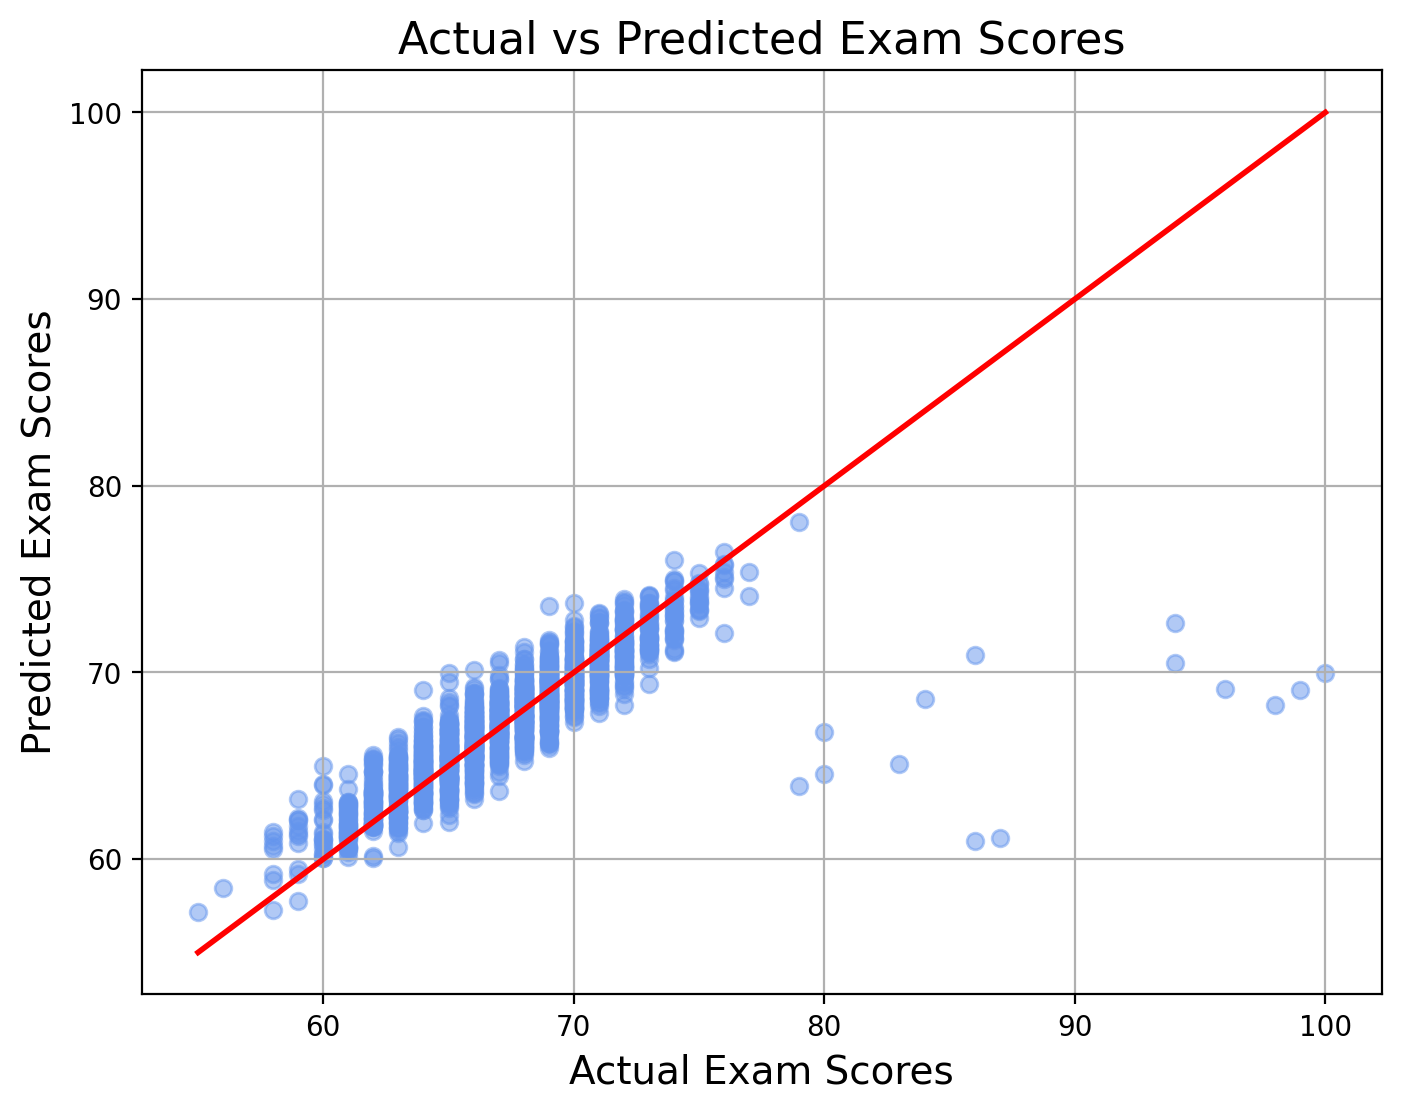
\includegraphics[width=\columnwidth]{5-actual-vs-predicted-scores.png}
  \caption{Predicted vs. observed exam scores}
  \label{5:actual-vs-predicted}
\end{figure}

At this point, we considered whether the observations that are very far from our line are influential points. An influence plot (Figure \ref{6:influence-plot}) shows us how there are just too many of these observations that fit the criteria to be considered an influential point (leverage higher than 3 times the mean leverage, statistically significant externally studentized residuals or Cook's distance higher than $\frac{4}{n}$, $n$ being the sample size).

We cannot simply treat these as outliers and remove them. We seem to not be considering that there are two distinct groups of students that should have different models.

\begin{figure}[h]
  \centering
  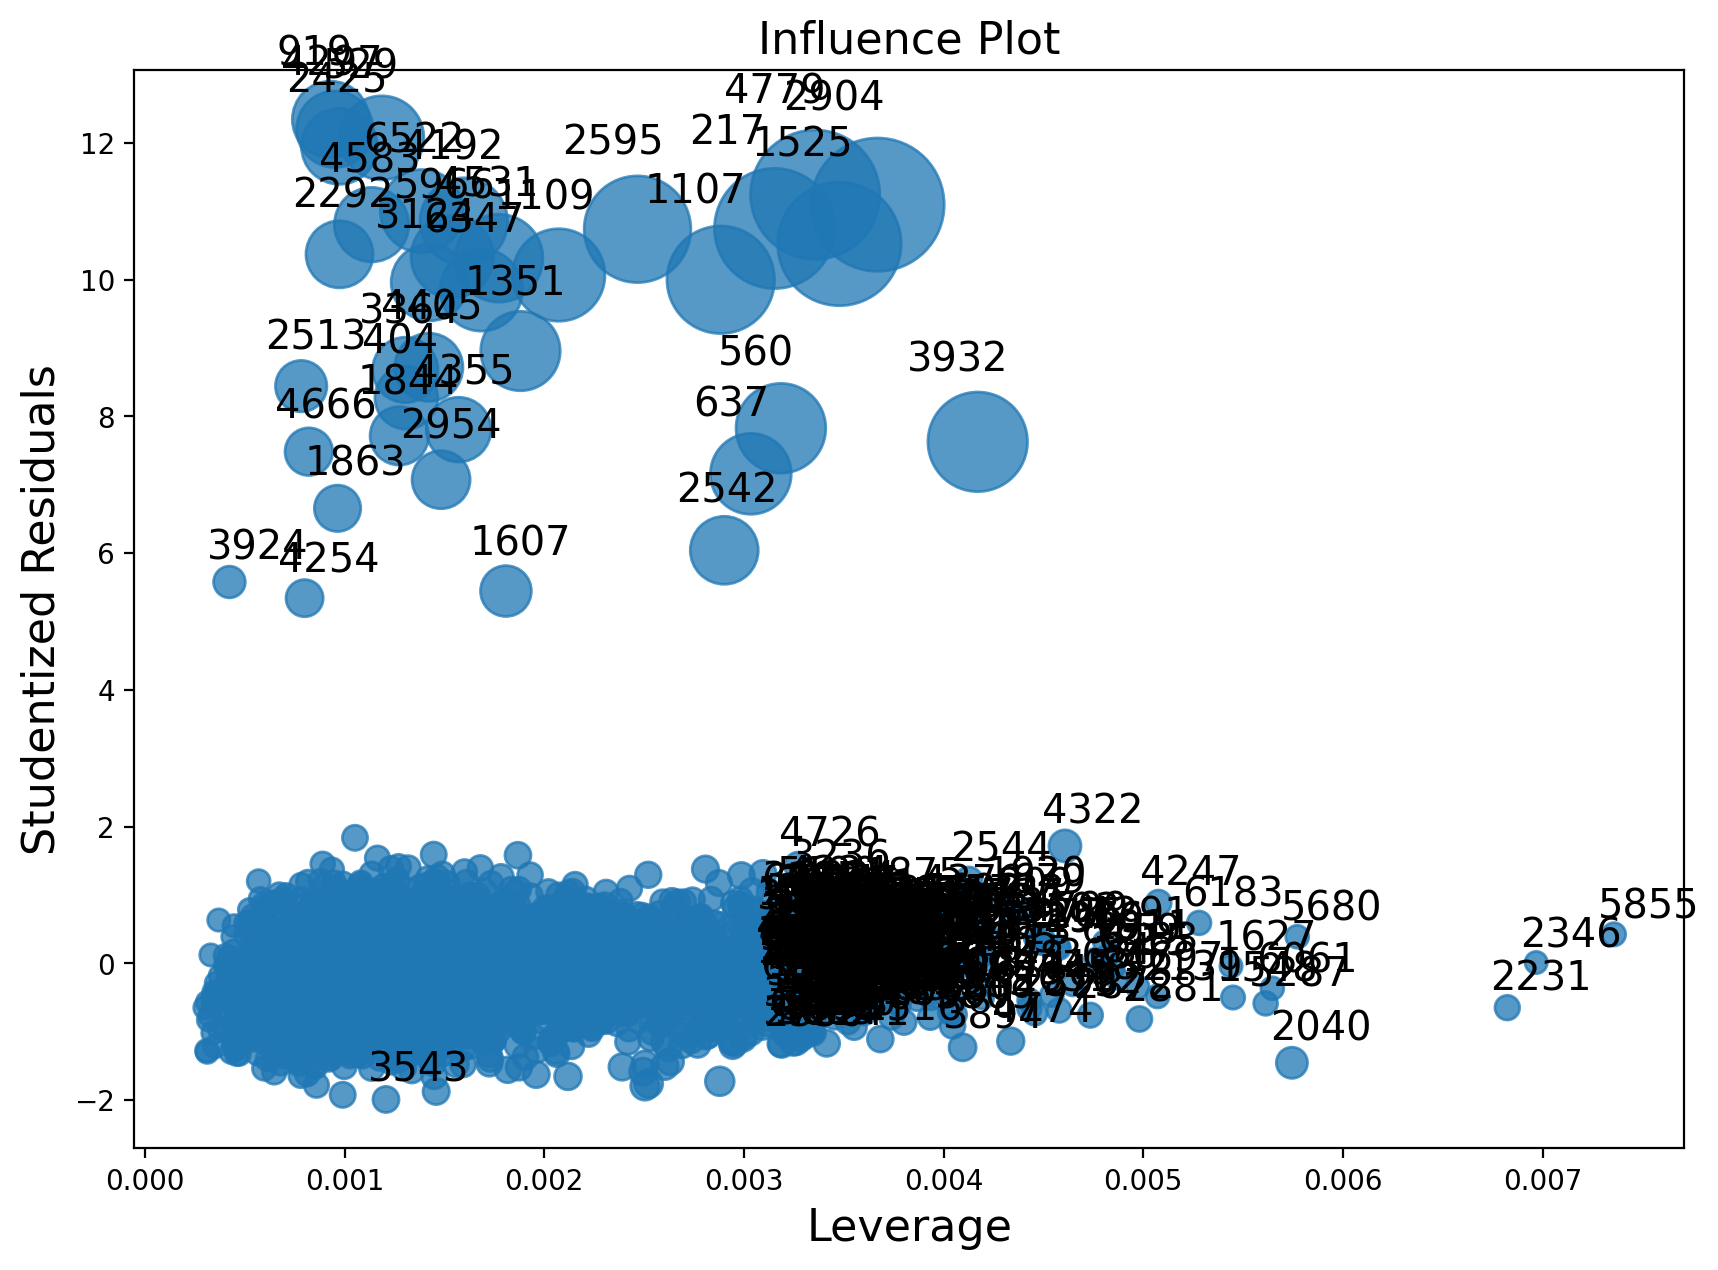
\includegraphics[width=\columnwidth]{6-influence-plot.png}
  \caption{Influence plot for the initial model}
  \label{6:influence-plot}
\end{figure}

To try and improve model fit, we performed a Box-Cox transformation on our model. The summary table for this initial model can be seen at Supplementary Figure \ref{fig:boxcox-model-summary}. After this, even if our metrics had improved ($R^2_a = 0.719$), our residual plot (Figure \ref{7:initial-residual}) showed that our strategy for modeling was not having success.

\begin{figure}[h]
  \centering
  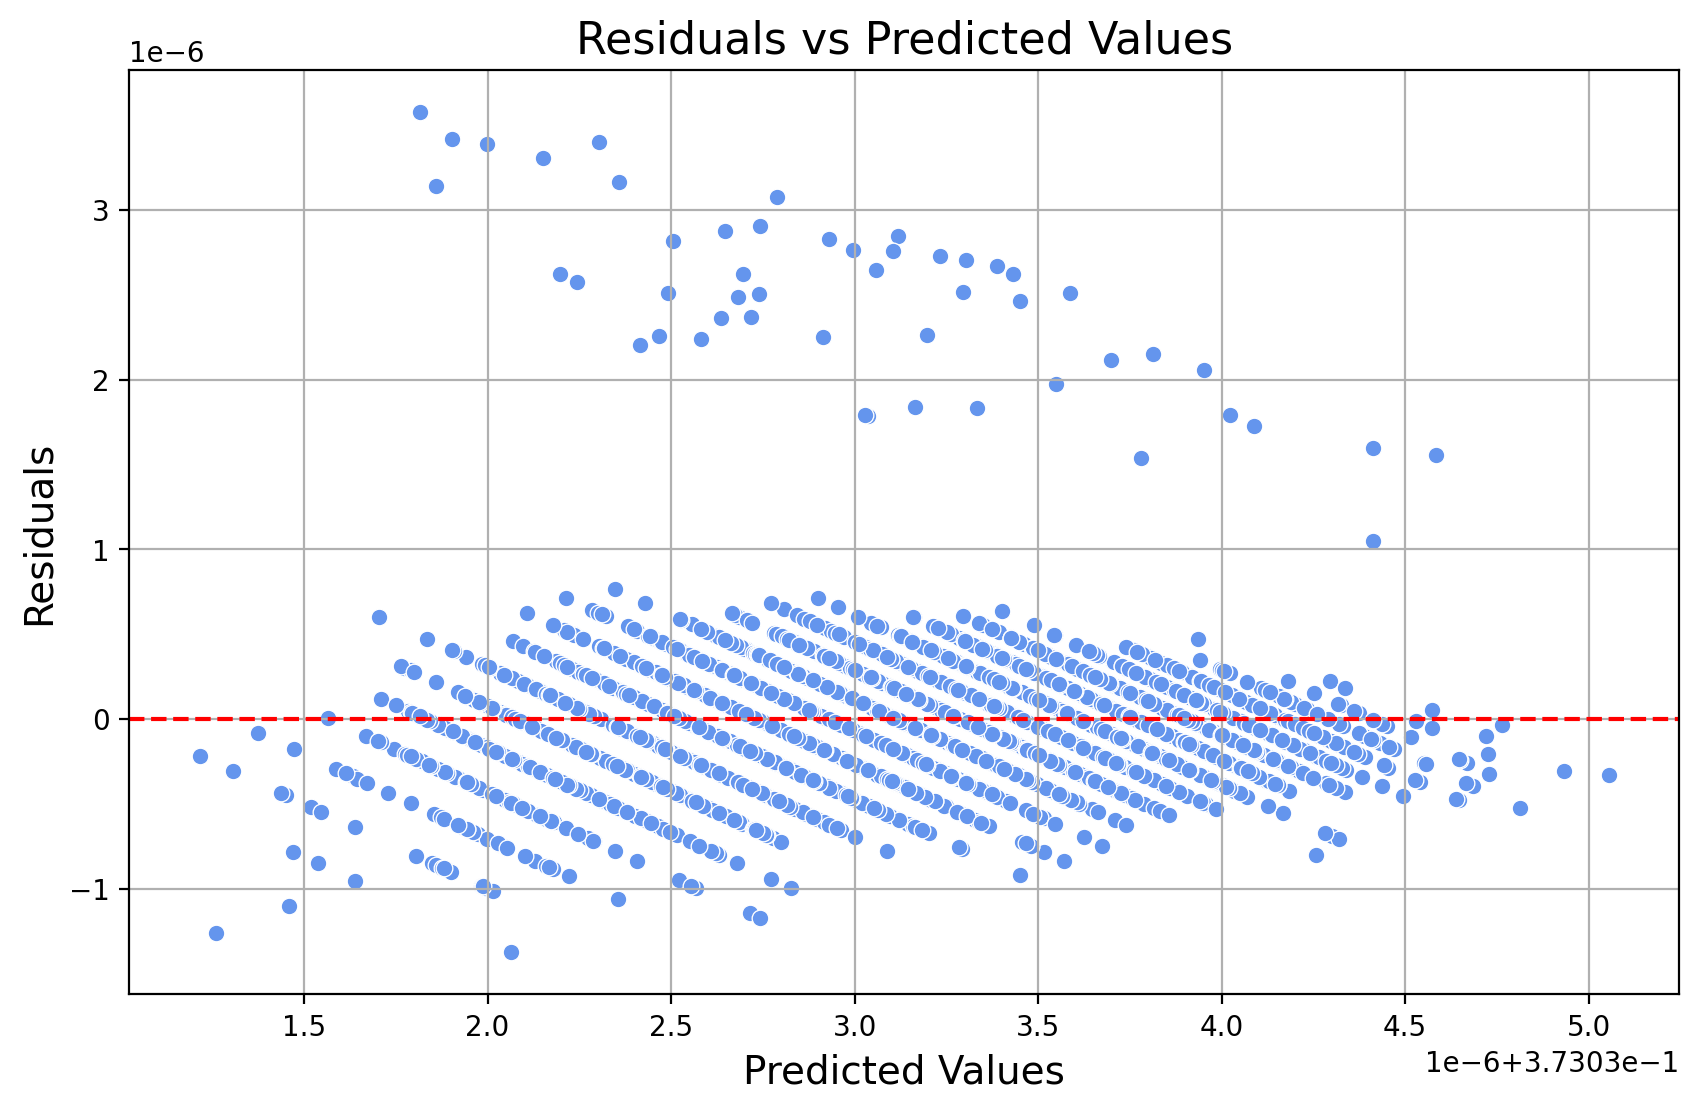
\includegraphics[width=\columnwidth]{7-residual-plot.png}
  \caption{Residual plot for the initial model.}
  \label{7:initial-residual}
\end{figure}

The residual plot showed that there still seemed to be a significant amount of data falling outside the expected bounds. We can clearly see that a chunk of our predictions have very high residuals, following what we could call a pattern.

This residual plot, an influence plot, and our discoveries regarding the Exam Scores variable during EDA, lead us to consider splitting the data.

\subsection*{Splitting the Data Into Two Models}
Since most of our observations have their exam scores clustered around 65\%, and we find a set of high performing students, we modeled performance under the assumption that these two student groups respond differently to predictors. and the predictors don't impact them in the same way. We decided to divide our dataset into two groups:
\begin{itemize}
  \item High Performing Students: Students with exam scores of 80 or above. (This will include students that achieve grades of B or higher).
  \item Average Performing Students: Students with exam scores under 80 (with grades from Fail until C+).
\end{itemize}
These two datasets were further divided into training and testing datasets.

We ended up with 6330 observations for the average performing students dataset, and 48 observations for the high performing students dataset. We acknowledge our high model will not have a high statistical power, seeing as training a model with only 48 observations limits accuracy. 

We will work extensively on our average performing students model, which includes the majority of the students on our dataset. We will also fit a model for the high performing students dataset, but since this is an under represented group in our dataset, we'd need more data to correctly assess student performance for students with high exam scores.

Our new approach to choose predictors involved the Lasso pipeline. LASSO (Least Absolute Shrinkage and Selection Operator) is an effective technique for handling situations with a large number of predictors and potential multicollinearity. It improves model performance by adding an L1 regularization term to the regression model, which penalizes the absolute size of the coefficients. This penalization has two key effects: first, it shrinks some coefficients toward zero, reducing the variance of the model and helping to prevent overfitting. Second, LASSO sets some coefficients exactly to zero, effectively selecting a subset of the most important predictors. By forcing less significant predictors to have a coefficient of zero, LASSO simplifies the model and ensures it retains only the most relevant features, thus improving interpretability and generalization to new data.

% RESULTS
\section{Results}
\subsection*{Low Scores Model}

The Lasso pipeline chose 10 predictors for this model:

\begin{itemize}
  \item Five categorical variables: access to resources, extracurricular activities, motivation level, family income, and parental education level.
  \item Five numerical variables: hours studied, attendance, previous scores, tutoring sessions, physical activity.
\end{itemize}

The summary table for the final \textbf{Low model} can be seen in Supplementary Table \ref{fig:low-model-summary}.

We can reference different model selection criteria to make sure this model is better and more accurate than our initial model (Table \ref{model-selection-low})

\begin{table}[ht]
  \begin{tabular}{|c|c|c|c|}
      \hline
      \textbf{Model} & \textbf{adj-$R^2$} & \textbf{AIC} & \textbf{BIC} \\ \hline
      Initial Model   & 0.600  & 2.077e+04  & 2.081e+04  \\ \hline
      Box-Cox Model   & 0.726  & -1.718e+05  & -1.718e+05  \\ \hline
      Low Model       & 0.898  & 1.511e+04  & 1.521e+04  \\ \hline
  \end{tabular}
  \caption{Model selection criteria: Initial model vs. Low model}
  \label{model-selection-low}
\end{table}

For this model, we achieve an adjusted R-squared of $0.898$, and the residual plot (Figure \ref{8:low-residual}) looks to be correctly scattered around the x-axis.

\begin{figure}[h]
  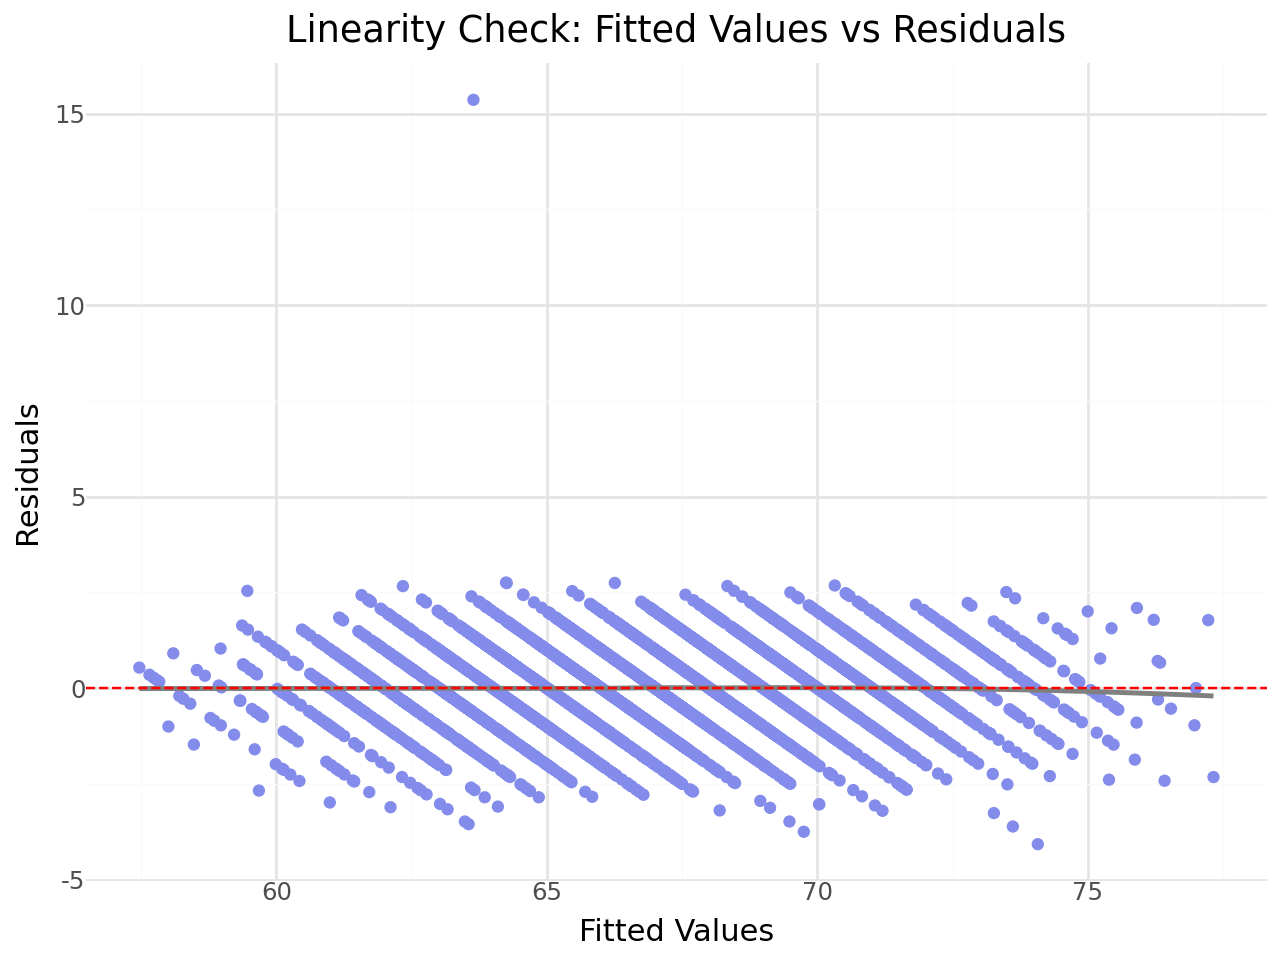
\includegraphics[width=0.9\columnwidth]{8-linearity-check.png}
  \caption{Residual plot for the low model.}
  \label{8:low-residual}
\end{figure}

The QQ-plot (Figure \ref{9:low-qq}) tells us the same story. We can see how most of our residuals almost perfectly fall on the regression line. This helps us confirm our model isn't violating any model assumptions, like the normality of the residuals.

\begin{figure}[h]
  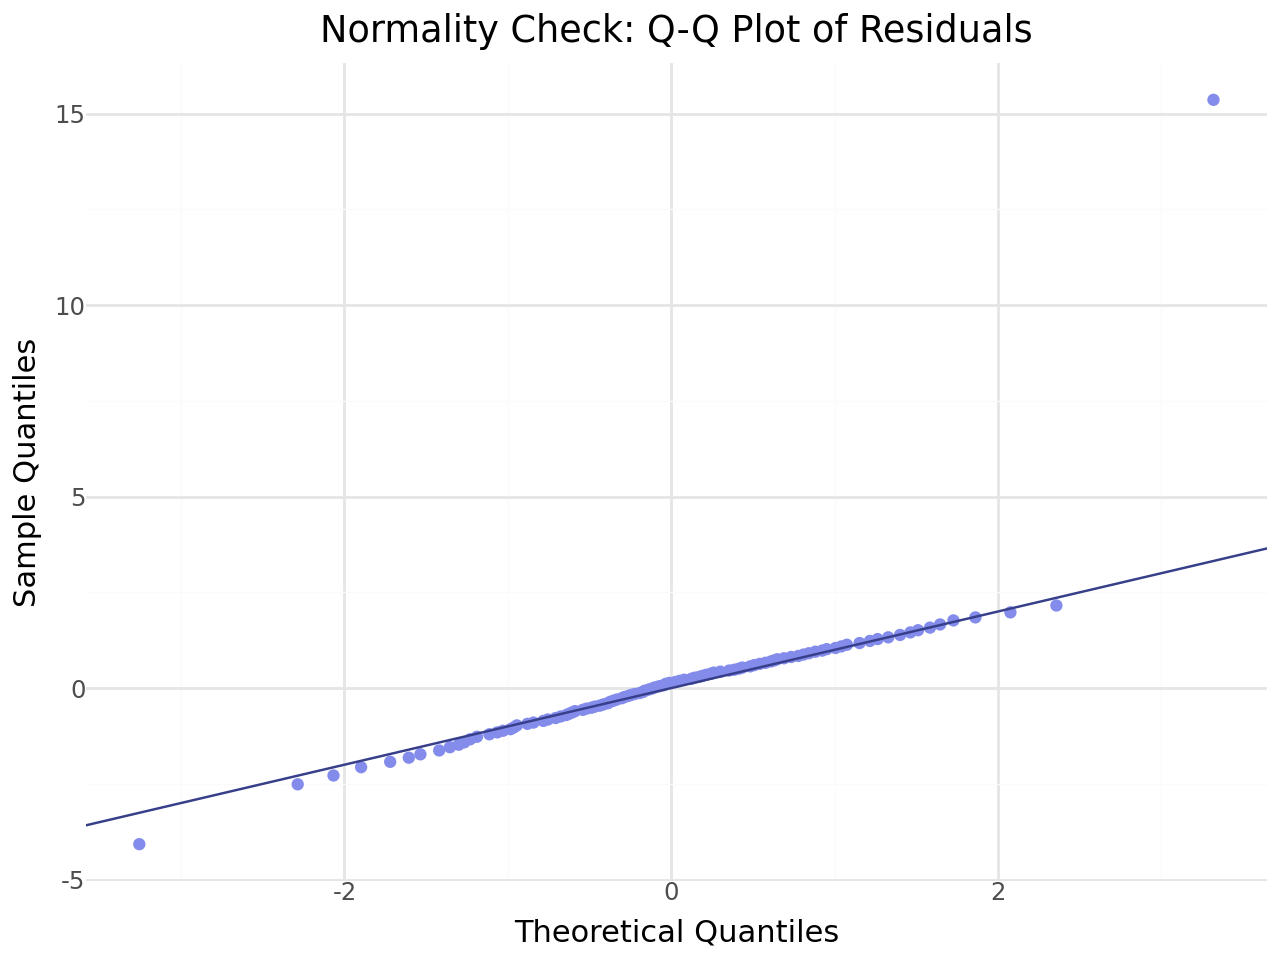
\includegraphics[width=0.9\columnwidth]{9-residual-qq-plot.png}
  \caption{QQ-plot for the low model.}
  \label{9:low-qq}
\end{figure}

Most of the data falls in the expected region, but we still see a few potential outliers. We decided to explore influential points to get a better look at these potential outliers.

Other diagnostic plots, like scatterplots of individual predictors vs response variable (Supplementary Figure \ref{10:predictors-scatterplot}) and correlation matrix (Supplementary Figure \ref{11:corr-heatmap}) can be seen on our supplementary material.

\subsubsection*{Influential Points}
To get a sense for the potential problematic observations in our data, we used three metrics: leverage, to get outliers, externally studentized residuals, to identify high discrepancy points, and Cook's distance, to definitely identify influence points.

In Table \ref{tab:influential-points} we can see that none of these metrics are high enough to flag the observations as influential points. Since this has no significant effect on our model, we'll leave them.

\begin{table}[H]
  \resizebox{\columnwidth}{!}{
  \begin{tabular}{|l|c|c|c|c|}
      \hline
      \textbf{Index} & \textbf{Leverage} & \textbf{Cook's Distance} & \textbf{Studentized Residual} \\
      \hline
      5043  & 0.007464   & $5.039074 \times 10^{-7}$ & -0.031705 \\ \hline
      53    & 0.006856   & 0.0004598461              & -0.999592 \\ \hline
      1002  & 0.006809   & 0.0005532396              & 1.100212  \\ \hline
  \end{tabular}
  }
  \caption{Leverage, Cook's Distance, and Studentized Residual for Selected Observations}
  \label{tab:influential-points}
\end{table}

Finally, we plotted our line of best fit with the residuals (Figure \ref{17:obs-vs-fitted}), to get a sense of how our model is performing.

\begin{figure}[h]
  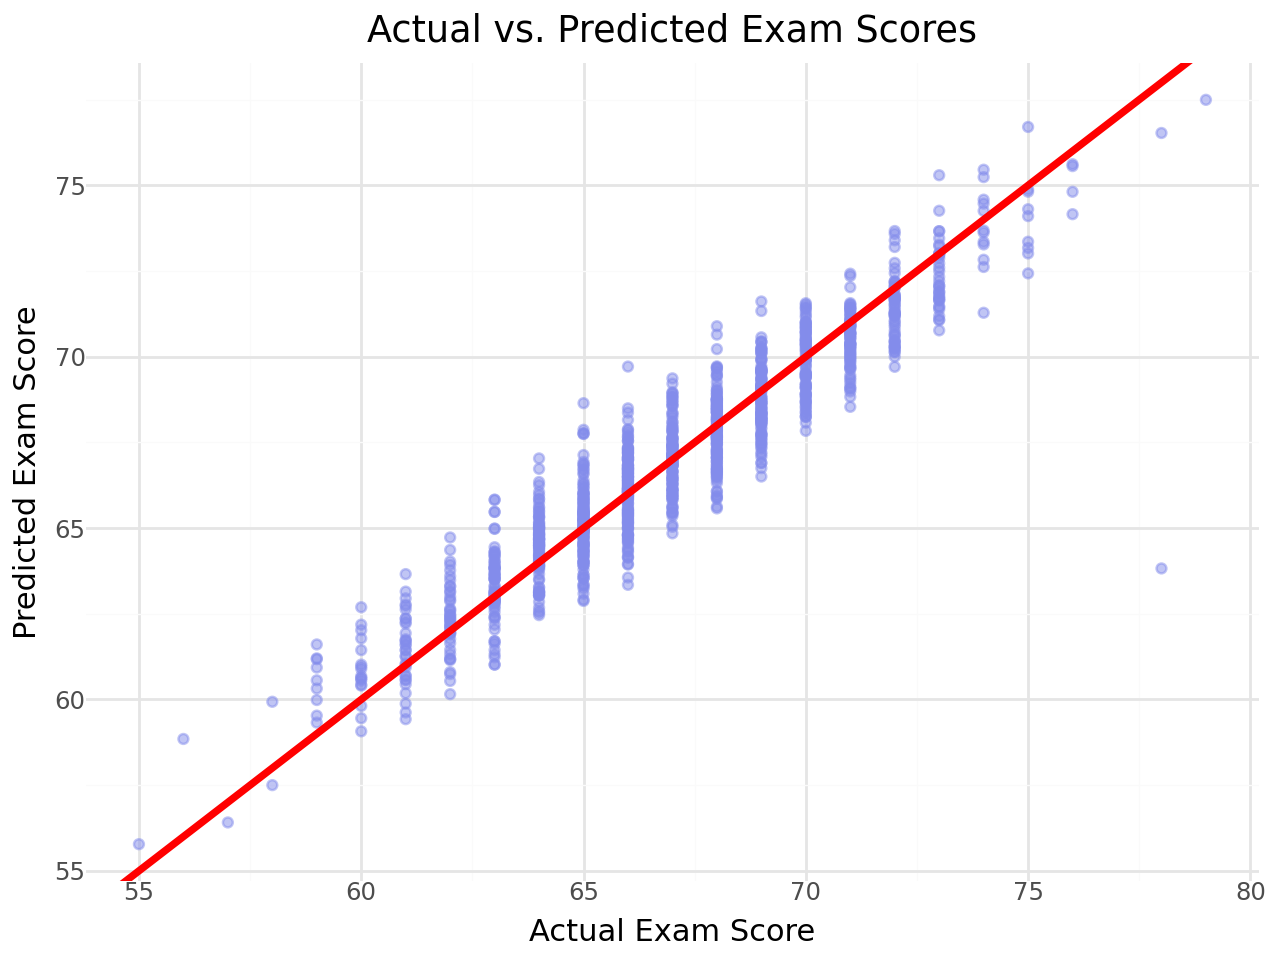
\includegraphics[width=\columnwidth]{17-observed-vs-fitted.png}
  \caption{Residual plot for the low model.}
  \label{17:obs-vs-fitted}
\end{figure}

We can see how all of the residuals fall in line with the line of best fit.

\subsection*{High Scores Model}

The Lasso pipeline chose 11 predictors for this model:

\begin{itemize}
  \item Six categorical variables: access to resources, internet access, family income, teacher quality, school type and parental education level.
  \item Five numerical variables: hours studied, attendance, sleep hours, previous scores and tutoring sessions.
\end{itemize}

The summary table for the final \textbf{High model} can be seen in Supplementary Table \ref{fig:high-model-summary}

As expected, the model's performance suggests that the available data may not be sufficient for achieving high accuracy. The \textbf{adjusted R-squared} value of $R^2_a = 0.602$ indicates that approximately 60.2\% of the variance in the response variable (exam score) is explained by the predictors in the model. While this suggests some predictive power, it is not particularly high.

The \textbf{AIC} of $229.6$ and \textbf{BIC} of $255.8$ are relatively high, suggesting that the model may not fit the data very well and that there could be some overfitting or inefficiency in the model, especially considering the limited number of observations (38).

Our \textbf{p-values} for most of the individual predictors are quite large, some being as high as $0.870$ (for physical activity). These high p-values suggest that many of the predictors are not statistically significant at common significance levels (such as $\alpha=0.05$). This implies that, individually, these predictors do not have a strong relationship with the response variable.

However, despite the lack of significance for individual predictors, the \textbf{F-test} p-value of $0.000541$ suggests that the model as a whole is statistically significant. This means that we can reject the null hypothesis that none of the predictors have any linear relationship with the response variable. In other words, while individual predictors may not show strong significance, the collective set of predictors likely explains some of the variance in exam score.

The diagnostic plots this time have less data to work with, but still don't show violation of our model assumptions. Our residuals seem to be randomly scattered around 0 (Figure \ref{18:linearity-check}), but we can also see that the variance it shows is very high, again confirming this model can have fairly high errors.

\begin{figure}[h]
  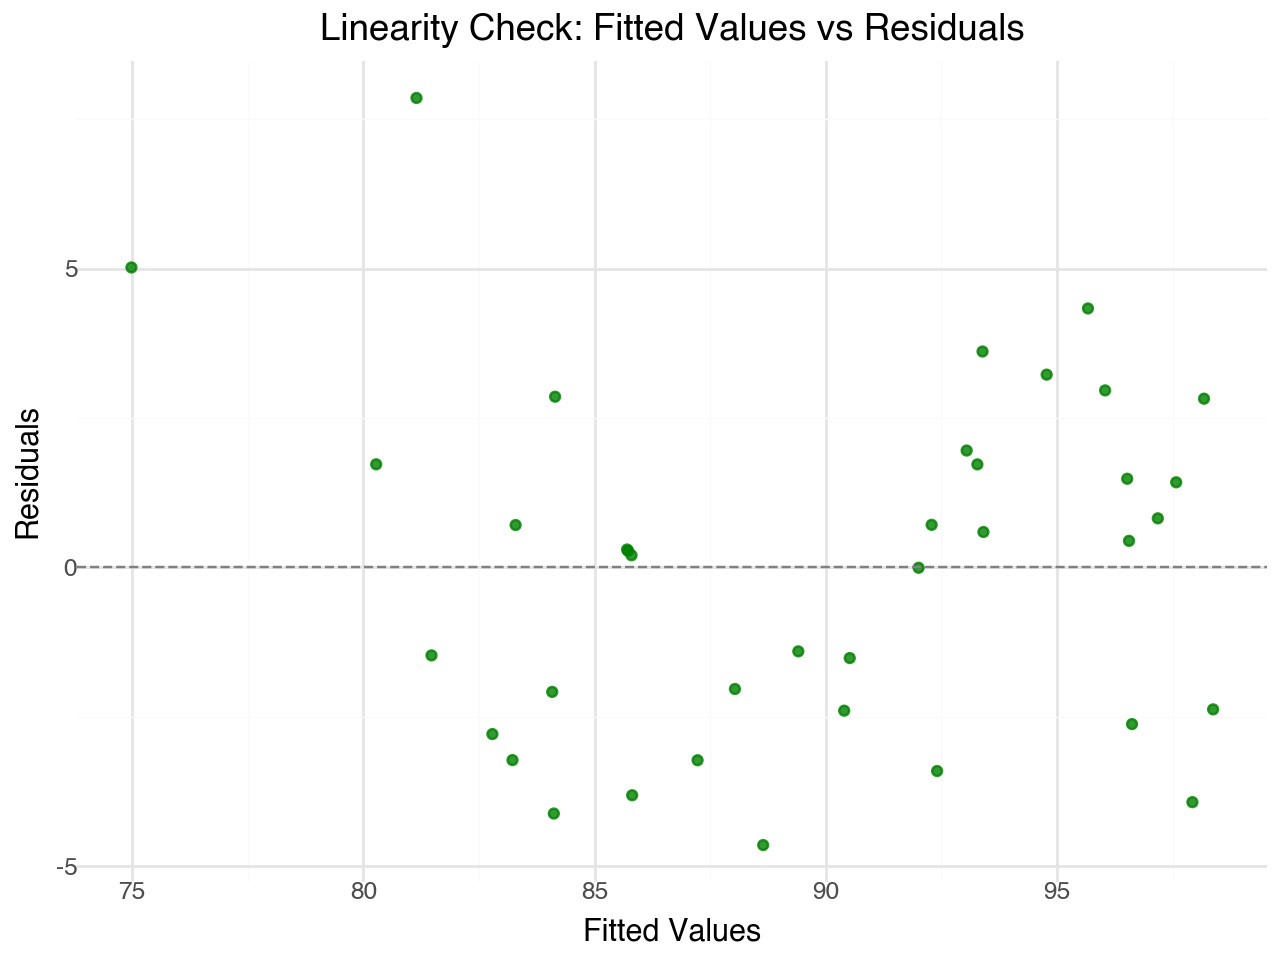
\includegraphics[width=\columnwidth]{18-linearity-check.png}
  \caption{Residual plot for the high model.}
  \label{18:linearity-check}
\end{figure}

The QQ-plot (Figure \ref{19:qq-plot}) also shows our theoretical and observed quantiles coinciding for the most part, but the residuals don't fall so much on the line compared to the low model.

\begin{figure}[h]
  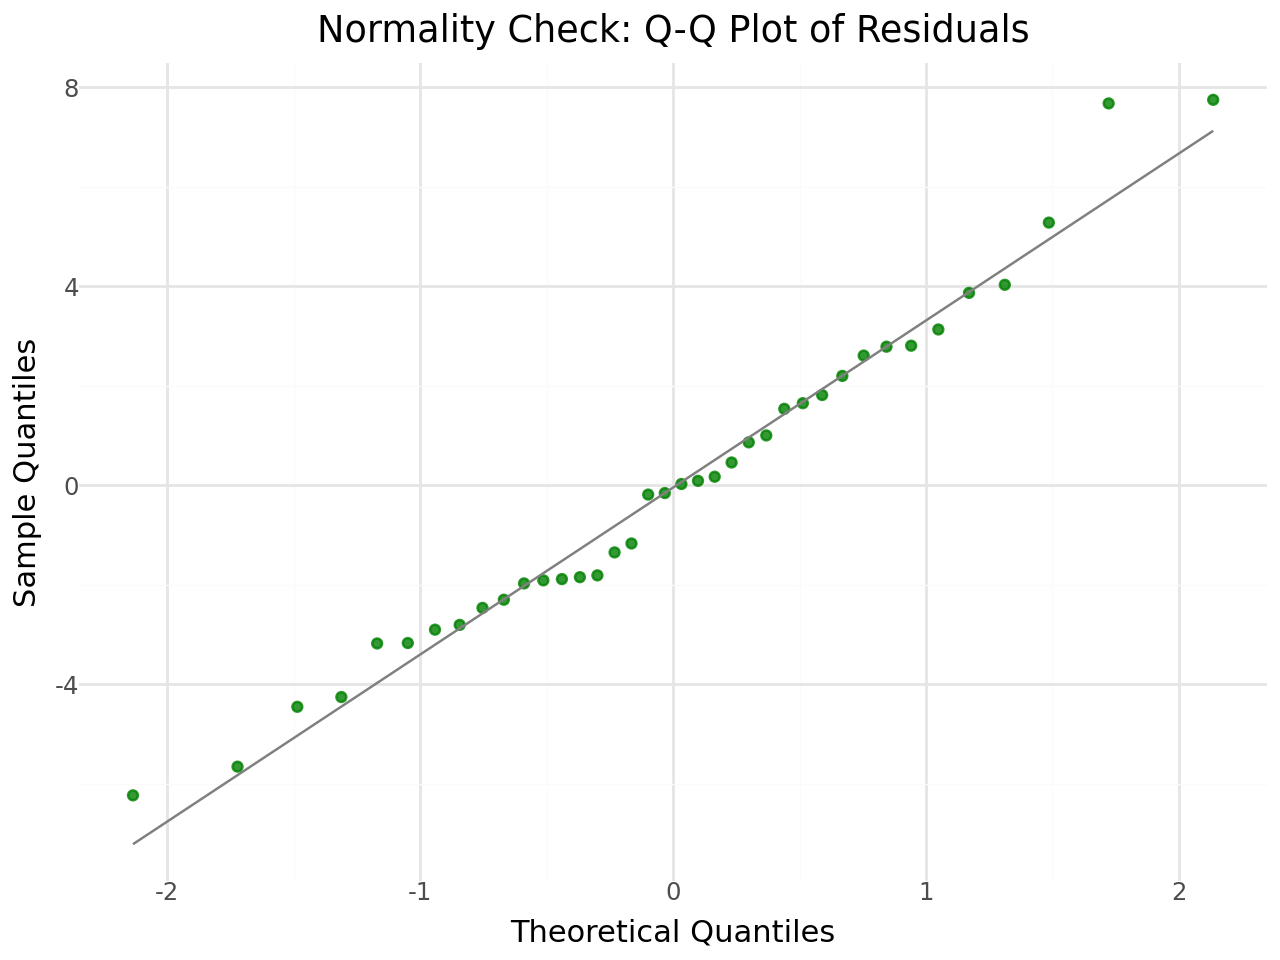
\includegraphics[width=\columnwidth]{19-qq-plot.png}
  \caption{QQ-plot for the high model.}
  \label{19:qq-plot}
\end{figure}

Other diagnostic plots, like scatterplots of individual predictors vs response variable (Supplementary Figure \ref{20:predictors-scatterplot}) and correlation matrix (Supplementary Figure \ref{21:corr-heatmap}) can be seen on our supplementary material.

In our plot for the actual vs. predicted exam scores for the high model (Figure \ref{22:observed-vs-fitted}) we can see that our residuals are very high and therefore, as predicted, our model does not have a lot of predicting power.

\begin{figure}[H]
  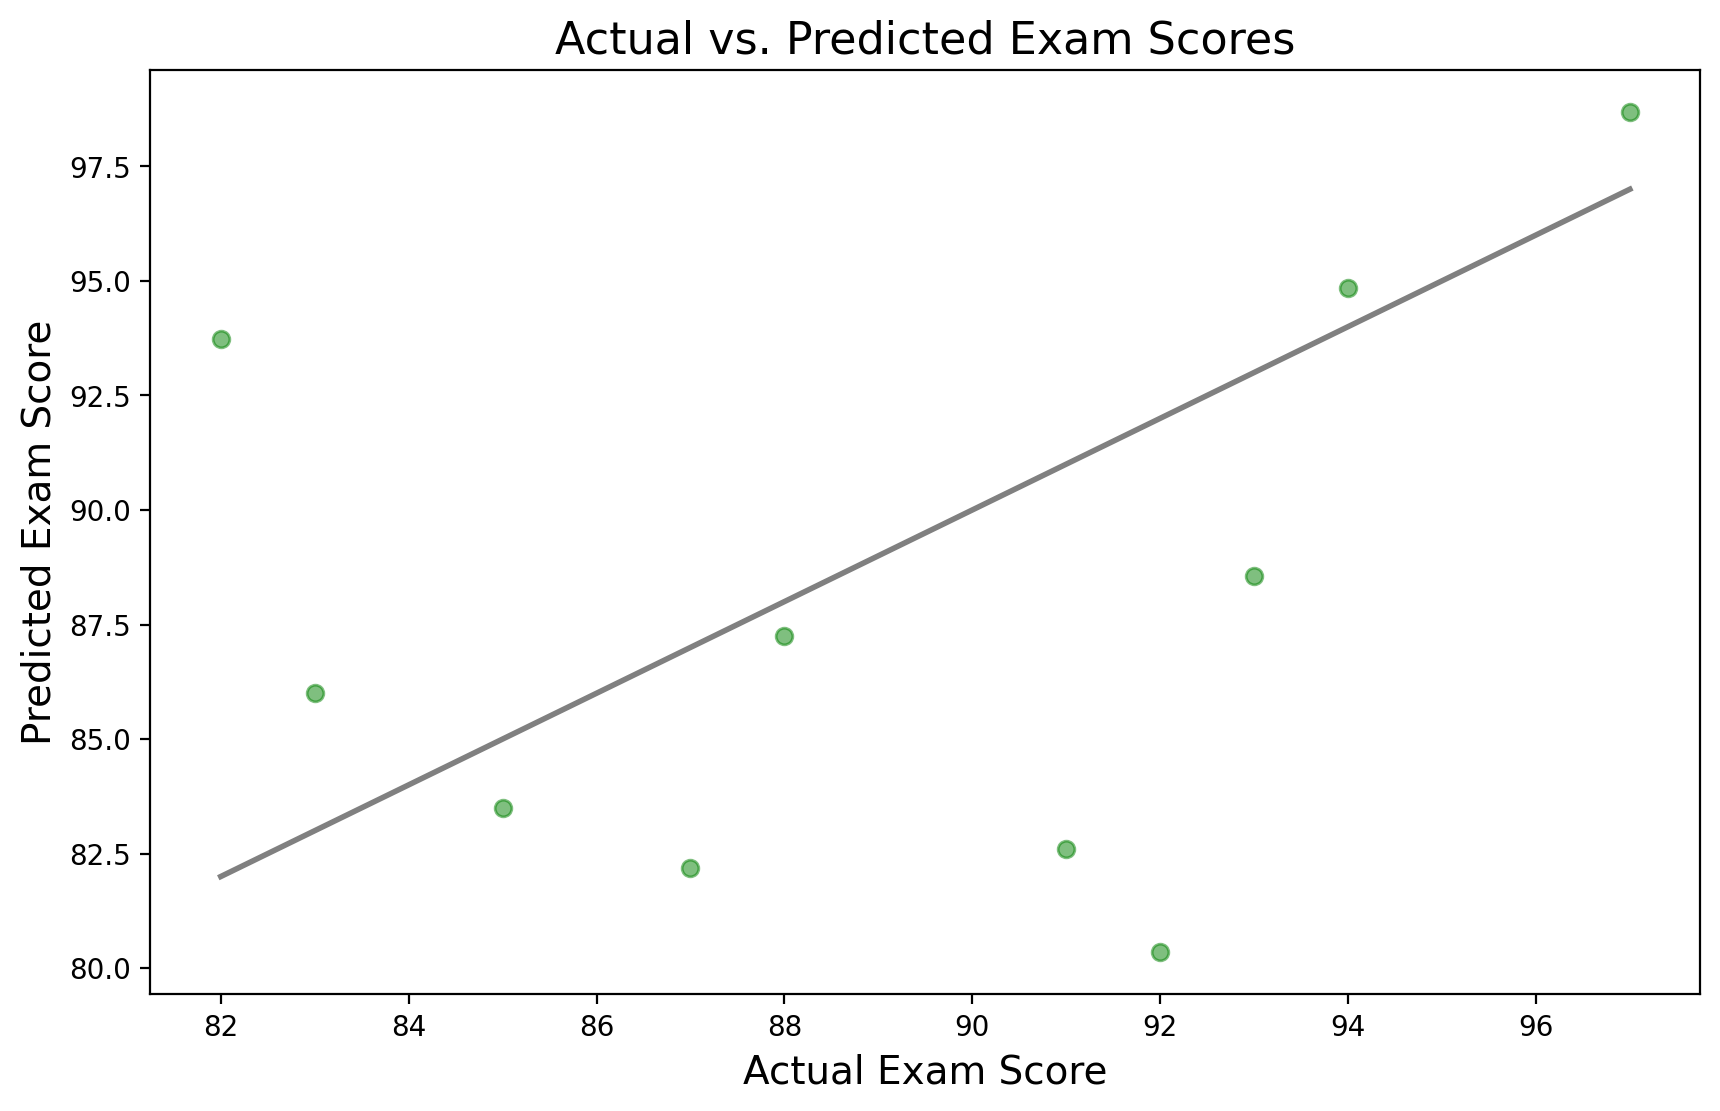
\includegraphics[width=\columnwidth]{22-observed-vs-fitted.png}
  \caption{Line of best fit: Actual vs. Predicted Exam Scores}
  \label{22:oberserved-vs-fitted}
\end{figure}

Gathering more data could help improve this particular model's accuracy and the significance of the individual predictors.

% DISCUSSION
\section{Discussion}

Our final MLR models predict student performace, measured as Exam Scores, based on a set of numerical and categorical predictors. We developed two separate models: one for students with average scores (below $80$) and another for high-performing students ($80$ or above). This split was necessary due to the clustering of most scores around $65\%$, with only a small subset of students in our dataset achieving high scores. After fitting an initial model with all of the observations, we could clearly see a different pattern between the predictors and the average scores vs. the high scores.

The adjusted $R^2$ for the average performance model was $0.898$, indicating a strong predictive ability. In contrast, the high-performance model achieved a lower adjusted $R^2$ of $0.602$, reflecting the limited predictive power for this group, due to the lack of data.

It is interesting to note which predictors ended up in each model (Table \ref{tab:predictor_selection}).

\begin{table}[h!]
  \centering
  \begin{tabular}{lcc}
  \hline
  \textbf{Predictor}                  & \textbf{Low Model} & \textbf{High Model} \\ 
  \hline
  Hours Studied                       & \ding{51} & \ding{51} \\
  Attendance                          & \ding{51} & \ding{51} \\
  Sleep Hours                         & \ding{55} & \ding{51} \\
  Previous Scores                     & \ding{51} & \ding{51} \\
  Tutoring Sessions                   & \ding{51} & \ding{51} \\
  Access to Resources                 & \ding{51} & \ding{51} \\
  Extracurricular Activities          & \ding{51} & \ding{55} \\
  Motivation Level                    & \ding{51} & \ding{55} \\
  Family Income                       & \ding{51} & \ding{51} \\
  Parental Education Level            & \ding{51} & \ding{51} \\
  Physical Activity                   & \ding{51} & \ding{55} \\
  Learning Disabilities               & \ding{55} & \ding{55} \\
  School Type                         & \ding{55} & \ding{51} \\
  Teacher Quality                     & \ding{55} & \ding{51} \\
  Internet Access                     & \ding{55} & \ding{51} \\
  Gender                              & \ding{55} & \ding{51} \\
  % st{Parental Involvement}             & \ding{55} & \ding{55} \\
  % st{Peer Influence}                  & \ding{55} & \ding{55} \\
  % st{Distance from Home}              & \ding{55} & \ding{55} \\
  \hline
  \end{tabular}
  \caption{Predictor selection for the average and high performance models.}
  \label{tab:predictor_selection}
\end{table}

This selection can already answer some of our research questions. We can see how Learning Disabilities was not picked out for any of the models, indicating that it does not affect a student's performance.

Predictors like hours studied, attendance, previous scores, tutoring sessions, access to resources, family income and parental education level have an impact for both of our models. We can go ahead and call these factors the ones that have the most significant impact in a student's performance.

We see positive coefficients for hours studied and attendance, indicating that the more hours a student studies and the more they attend lessons, the higher they'll score on their exams.

For the access to resources, a lower coefficient for the Low and Medium levels compared to the High level indicates how the less access a student has to resources, the more their performance will suffer. A similar behavior can be concluded for the family income variable. The lower the family income, the lower the student's exam scores. This answers our question about how socioeconomic factors pertaining to a student or their family impacts their performance. The lower the income and access to resources, the more the student's grades decrease.

In regards to a student's parents' education level, we can see how having chosen College as the baseline, our models indicate that for parental education level of High School the student's exam scores are on average 0.47 points lower, and for the Postgraduate level they're 0.53 points higher instead. This shows us how having educated parents is an indicator of a student performing better in exams.

We can see however that different predictors were chosen to model performance for our two groups of students.

\subsection*{Specific predictors for the Average Performing Students Model (Low Model)}
For average performing students, we have predictors that don't seem to influence exam scores for high performing students, like extracurricular activities, motivation level, or physical activity.

Looking at our model, we can see how a student participating in extracurricular activities will make them score 0.46 better on average compared to a student who doesn't.

We can also clearly see how motivation level has a clear impact on exam scores, the coefficient for the dummy variable T.Medium indicating a decrease in score of 0.44, and for T.Low of 0.96 compared to students with motivation level high.


% CONCLUSION
\section{Conclusion}

We were able to identify several factors that significantly impacted student performance, with the most significant predictors being hours studied, attendance, prior academic performance, and motivation. The high-performance model, despite being less robust, also indicates that these same factors may influence students achieving top scores. 

These findings also help to identify areas where educators and policymakers can create significant changes. By increasing study hours, boosting attendance, and providing tutoring sessions, educators will see an improvement in student exam scores. Additionally, factors like access to resources and parental education play a meaningful role, suggesting that there's another avenue for educators to identify students who may require early intervention. 

Future research focusing on high-performing students would help to improve model accuracy and predictive power. Including other variables such as mental health or learning environments could also help to capture additional aspects of student performance. Overall, this underscores the value of data-driven strategies in education and provides a foundation into further exploration on how to optimize students' academic success.

\section{Data and Code Availability}
All of the code and data for this project can be found on our \href{https://github.com/cztm/linear-regression}{Git Repository}.

\newpage
\onecolumn

\section*{Supplementary Materials}

\renewcommand{\figurename}{Supplementary Figure}
\setcounter{figure}{0}

\begin{figure*}[h]
  \centering
  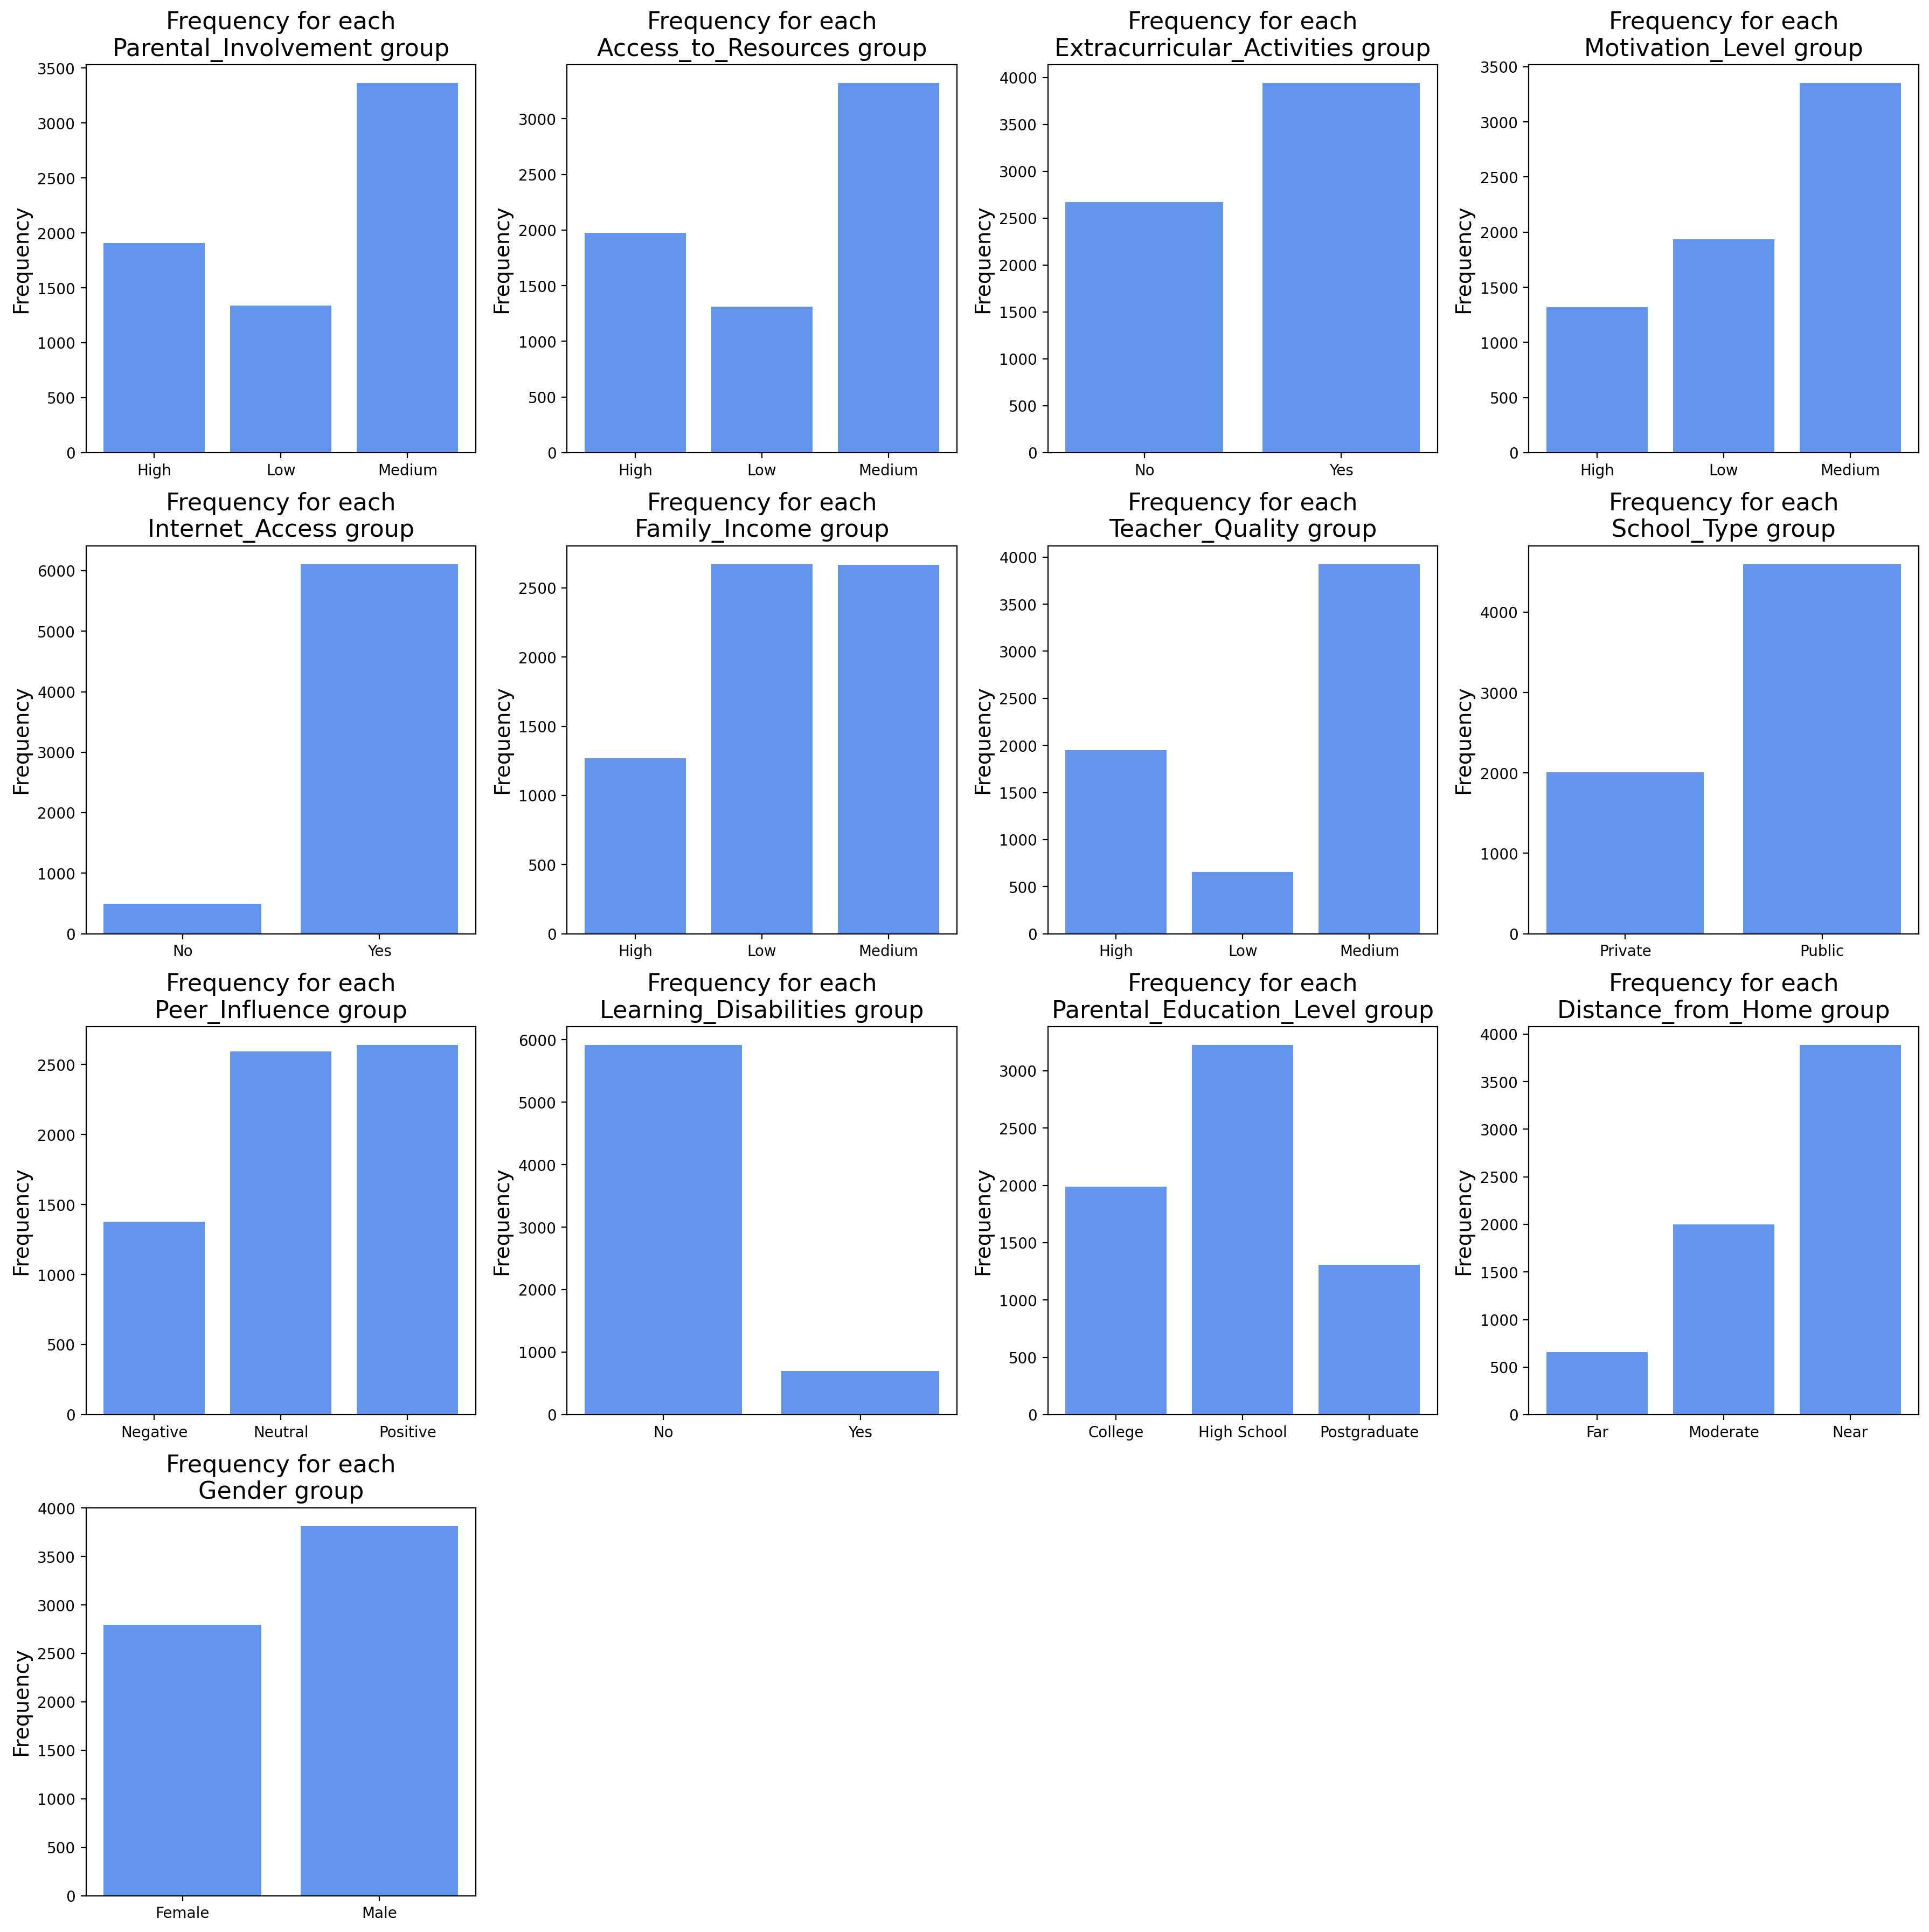
\includegraphics[width=0.9\columnwidth]{1-barplots.png}
  \caption{Plotting the frequency of each category for our categorical variables.}
  \label{1:barplots}
\end{figure*}

\newpage
\renewcommand{\tablename}{Supplementary Table}
\setcounter{table}{0}

\begin{table*}[ht]
  \centering
  \begin{tabular}{|c|c|c|c|}
      \hline
      \textbf{Parental Involvement/Access to Resources} & \textbf{High} & \textbf{Low} & \textbf{Medium} \\ \hline
      High   & 568  & 413  & 927  \\ \hline
      Low    & 414  & 231  & 692  \\ \hline
      Medium & 993  & 669  & 1700 \\ \hline
  \end{tabular}
  \caption{Confusion table: Parental Involvement vs. Access to Resources.}
  \label{tab:confusion1}
\end{table*}

\begin{table*}[ht]
  \centering
  \begin{tabular}{|c|c|c|c|}
      \hline
      \textbf{Peer Influence/Family Income} & \textbf{High} & \textbf{Low} & \textbf{Medium} \\ \hline
      Negative & 251 & 577 & 549 \\ \hline
      Neutral  & 493 & 1038 & 1061 \\ \hline
      Positive & 525 & 1057 & 1056 \\ \hline
  \end{tabular}
  \caption{Confusion table: Family Income vs. Peer Influence.}
  \label{tab:confusion2}
\end{table*}

\begin{table*}[ht]
  \centering
  \begin{tabular}{|c|c|c|c|}
      \hline
      \textbf{Distance from home/Motivation Level} & \textbf{High} & \textbf{Low} & \textbf{Medium} \\ \hline
      Far       & 142   & 185   & 331   \\ \hline
      Moderate  & 394   & 611   & 993   \\ \hline
      Near      & 773   & 1125  & 1986  \\ \hline
  \end{tabular}
  \caption{Confusion table: Motivation Level vs. Distance from Home.}
  \label{tab:confusion3}
\end{table*}

\renewcommand{\figurename}{Supplementary Figure}
\setcounter{figure}{1}

\begin{figure*}[h]
  \centering
  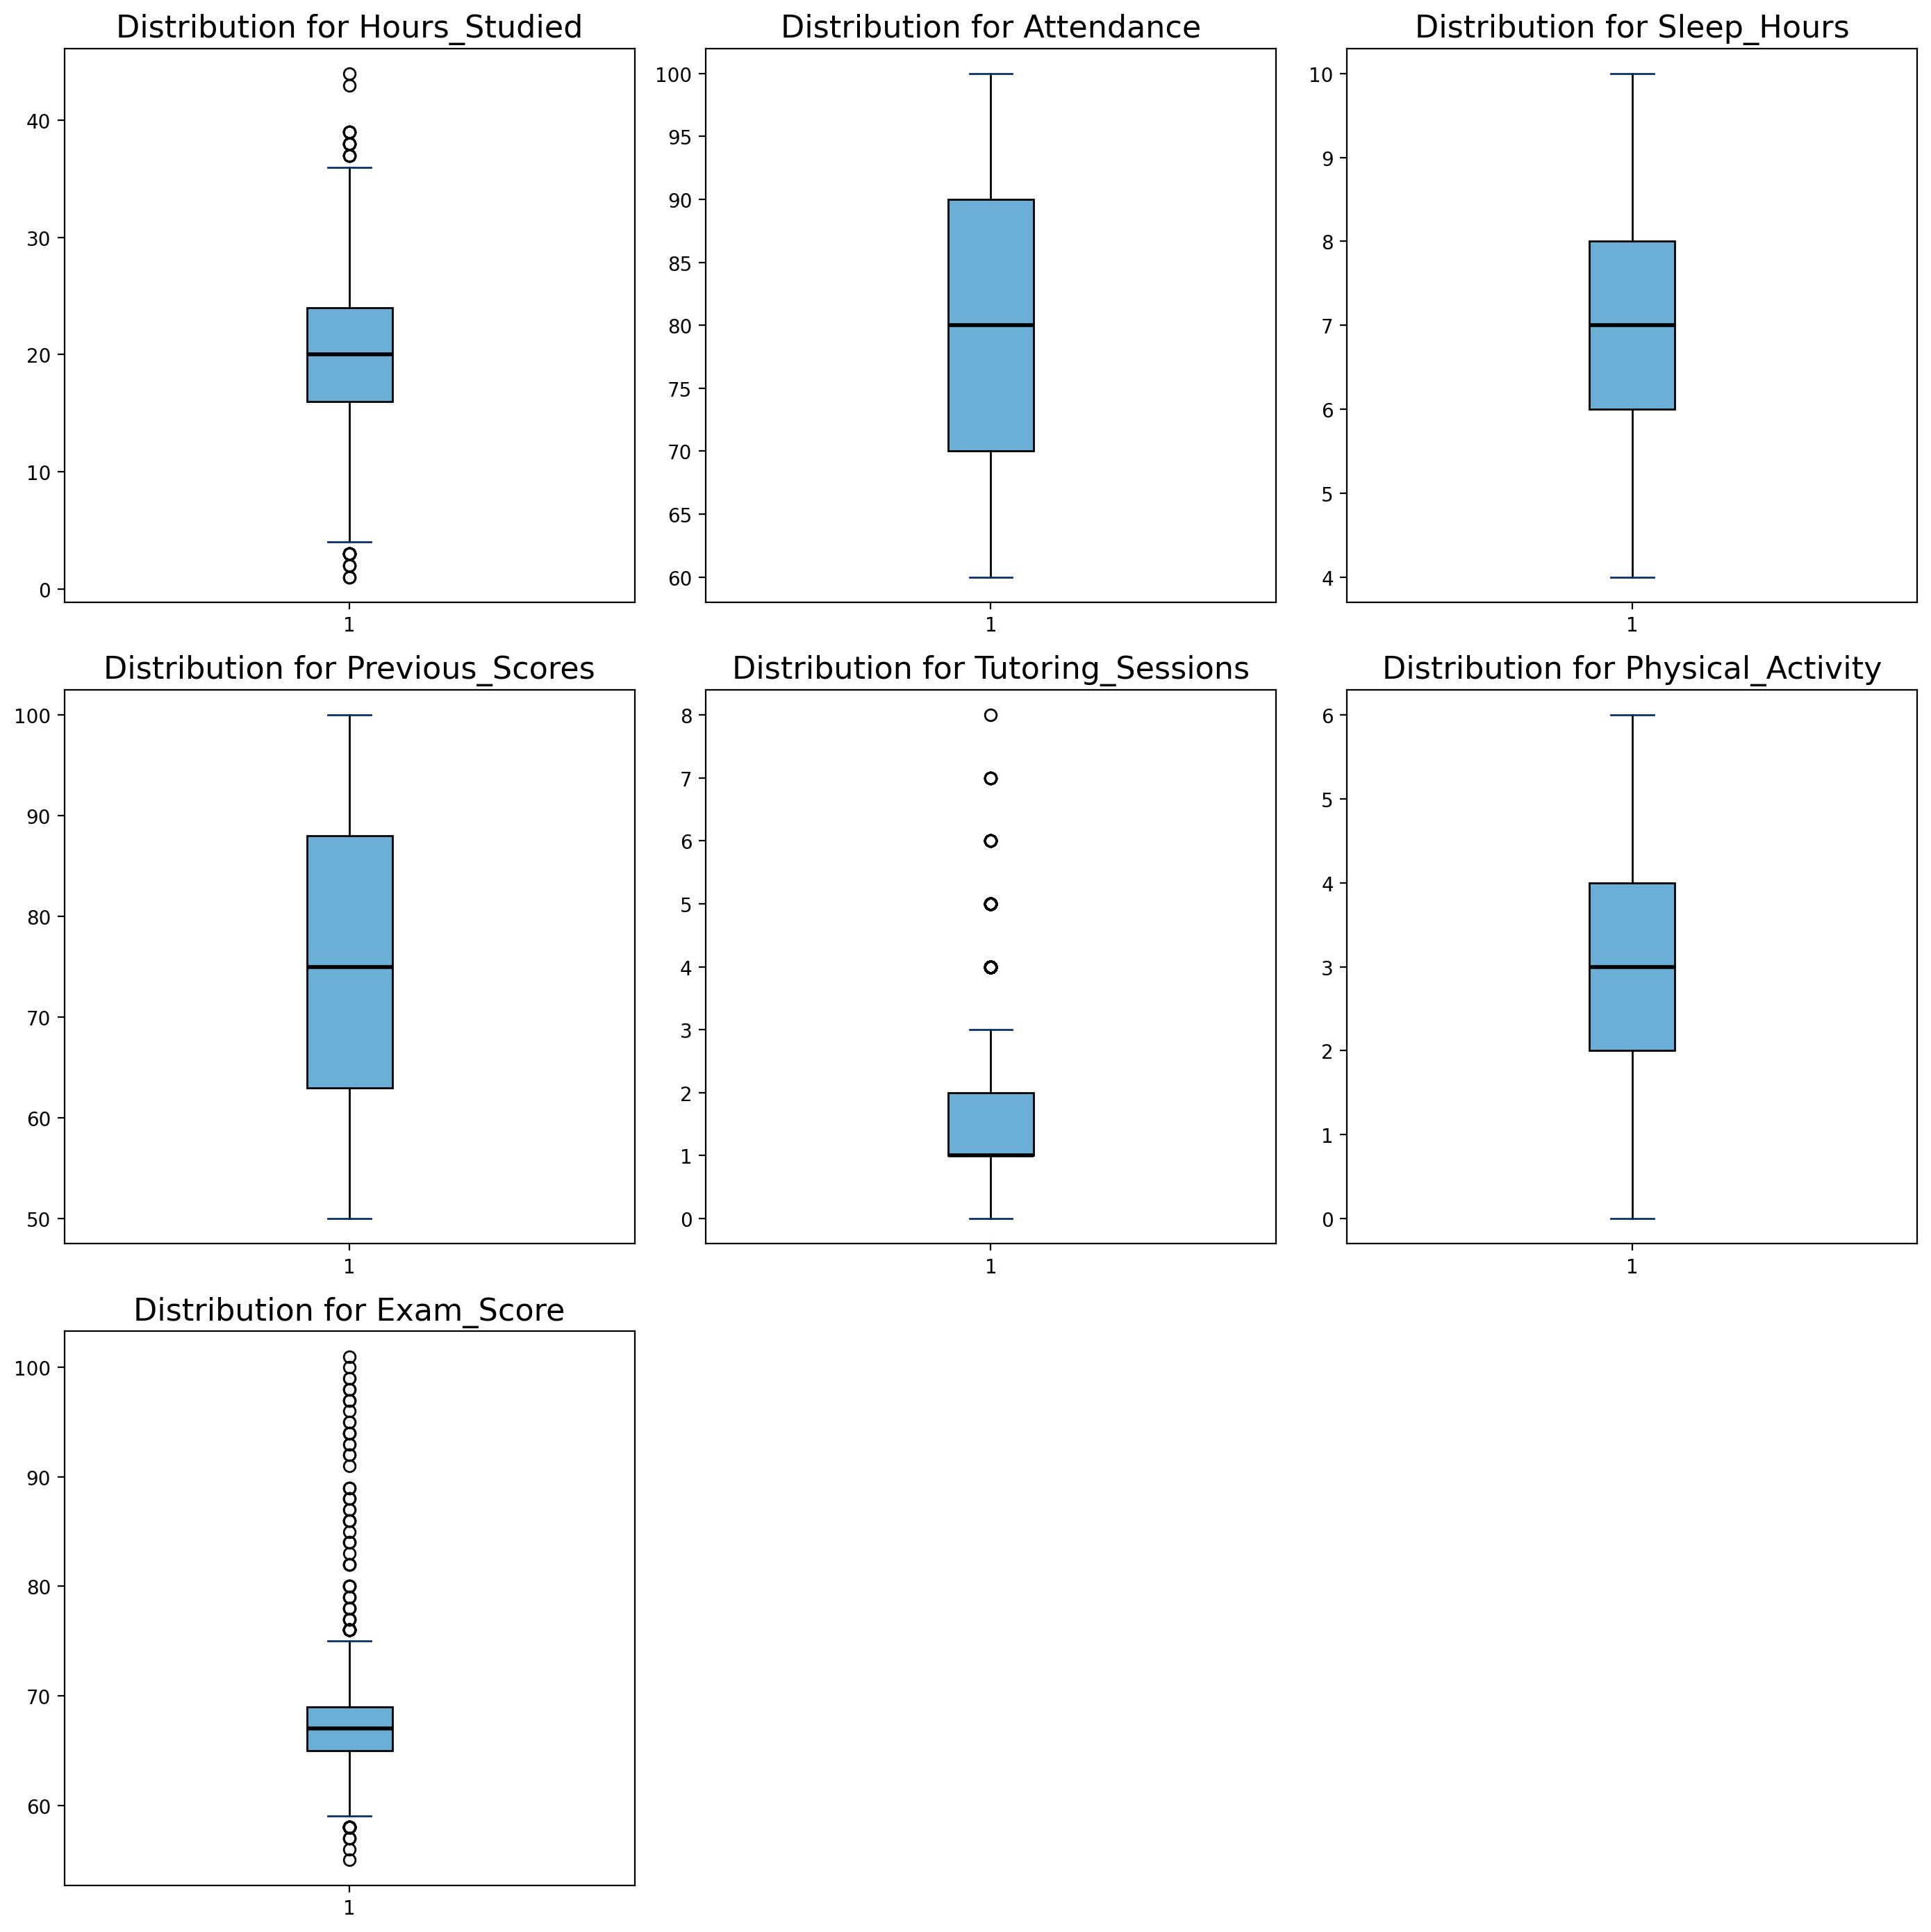
\includegraphics[width=0.9\columnwidth]{2-boxplots.png}
  \caption{Plotting the distribution of each numerical variable.}
  \label{2:boxplots}
\end{figure*}

\begin{figure*}[h]
  \centering
  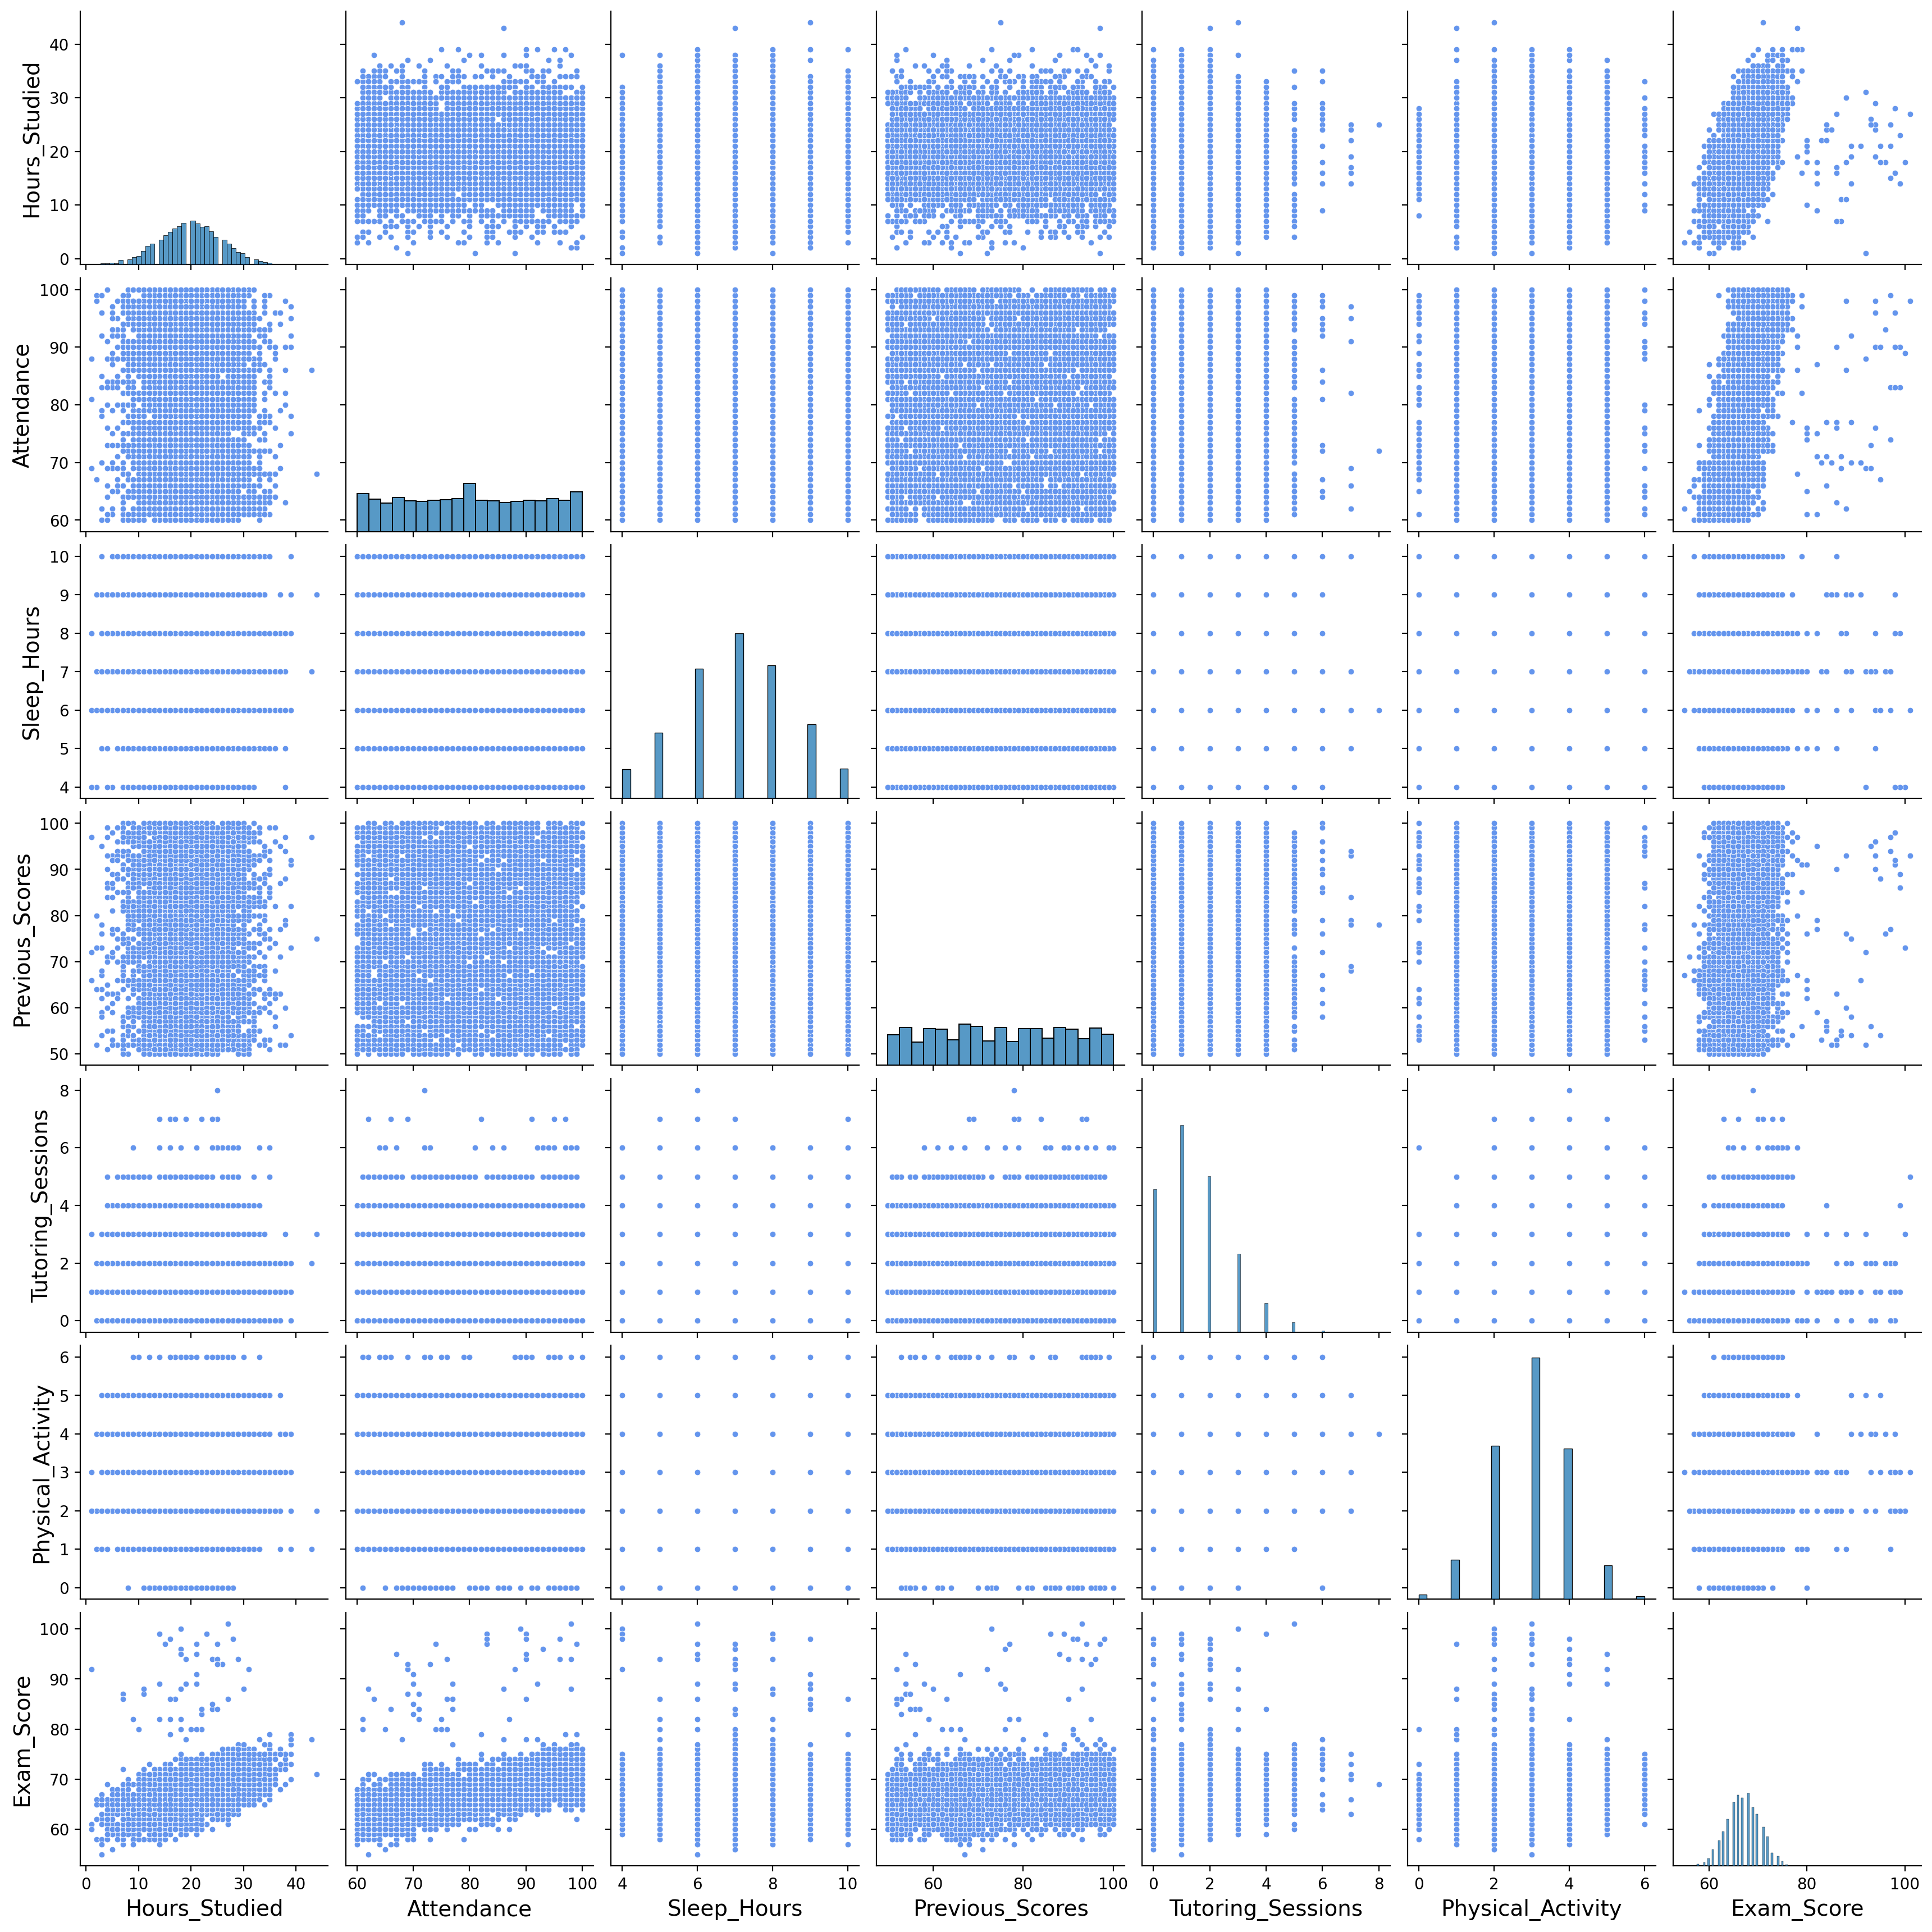
\includegraphics[width=0.9\columnwidth]{3-pairwise-plot.png}
  \caption{Numerical variable pairwise plot: Initial assessment of linear relationships between our variables.}
  \label{3:pairwise}
\end{figure*}

\begin{figure*}[ht]
  \centering
  \begin{Verbatim}[commandchars=\\\{\}]
                                      OLS Regression Results
          ==============================================================================
          Dep. Variable:             Exam\_Score   R-squared:                       0.601
          Model:                            OLS   Adj. R-squared:                  0.600
          Method:                 Least Squares   F-statistic:                     1117.
          Date:                Fri, 11 Oct 2024   Prob (F-statistic):               0.00
          Time:                        19:14:45   Log-Likelihood:                -10378.
          No. Observations:                4464   AIC:                         2.077e+04
          Df Residuals:                    4457   BIC:                         2.081e+04
          Df Model:                           6
          Covariance Type:            nonrobust
          ==============================================================================
          coef    std err          t      P>|t|      [0.025      0.975]
          ------------------------------------------------------------------------------
          const         67.2581      0.037   1815.017      0.000      67.185      67.331
          x1             2.2684      0.037     61.190      0.000       2.196       2.341
          x2             1.7595      0.037     47.445      0.000       1.687       1.832
          x3             0.6932      0.037     18.689      0.000       0.620       0.766
          x4             0.5972      0.037     16.108      0.000       0.524       0.670
          x5             0.3913      0.037     10.554      0.000       0.319       0.464
          x6            -0.3301      0.037     -8.905      0.000      -0.403      -0.257
          ==============================================================================
          Omnibus:                     5636.291   Durbin-Watson:                   1.996
          Prob(Omnibus):                  0.000   Jarque-Bera (JB):           918821.456
          Skew:                           6.918   Prob(JB):                         0.00
          Kurtosis:                      71.909   Cond. No.                         1.05
          ==============================================================================

          Notes:
          [1] Standard Errors assume that the covariance matrix of the errors is correctly
          specified.
  \end{Verbatim}
  \caption{Summary of Regression Results for the Initial Model}
  \label{fig:initial-model-summary}
\end{figure*}

\begin{figure*}[ht]
  \centering
  \begin{Verbatim}[commandchars=\\\{\}]
                                      OLS Regression Results
          ==============================================================================
          Dep. Variable:                      y   R-squared:                       0.726
          Model:                            OLS   Adj. R-squared:                  0.726
          Method:                 Least Squares   F-statistic:                     2814.
          Date:                Fri, 11 Oct 2024   Prob (F-statistic):               0.00
          Time:                        19:15:00   Log-Likelihood:                 85921.
          No. Observations:                6378   AIC:                        -1.718e+05
          Df Residuals:                    6371   BIC:                        -1.718e+05
          Df Model:                           6
          Covariance Type:            nonrobust
          ==============================================================================
                          coef    std err          t      P>|t|      [0.025      0.975]
          ------------------------------------------------------------------------------
          const          0.3730   4.28e-09   8.72e+07      0.000       0.373       0.373
          x1          4.163e-07   4.28e-09     97.329      0.000    4.08e-07    4.25e-07
          x2          3.176e-07   4.28e-09     74.239      0.000    3.09e-07    3.26e-07
          x3          1.255e-07   4.28e-09     29.325      0.000    1.17e-07    1.34e-07
          x4          1.095e-07   4.28e-09     25.609      0.000    1.01e-07    1.18e-07
          x5          7.219e-08   4.28e-09     16.877      0.000    6.38e-08    8.06e-08
          x6         -5.812e-08   4.28e-09    -13.590      0.000   -6.65e-08   -4.97e-08
          ==============================================================================
          Omnibus:                     4705.241   Durbin-Watson:                   1.997
          Prob(Omnibus):                  0.000   Jarque-Bera (JB):           189213.016
          Skew:                           3.100   Prob(JB):                         0.00
          Kurtosis:                      28.953   Cond. No.                         1.05
          ==============================================================================
          
          Notes:
          [1] Standard Errors assume that the covariance matrix of the errors is correctly
          specified.
  \end{Verbatim}
  \caption{Summary of Regression Results for the Initial Model after Box Cox transformation}
  \label{fig:boxcox-model-summary}
\end{figure*}

\begin{figure*}[ht]
  \centering
  
  % First Table
  \begin{subtable}{\textwidth}
    \centering
    \begin{tabular}{lclc}
      \toprule
      \textbf{Dep. Variable:}                             &   Exam\_Score    & \textbf{  R-squared:         } &     0.898   \\
      \textbf{Model:}                                     &       OLS        & \textbf{  Adj. R-squared:    } &     0.898   \\
      \textbf{Method:}                                    &  Least Squares   & \textbf{  F-statistic:       } &     3183.   \\
      \textbf{Date:}                                      & Sat, 12 Oct 2024 & \textbf{  Prob (F-statistic):} &     0.00    \\
      \textbf{Time:}                                      &     22:32:24     & \textbf{  Log-Likelihood:    } &   -7540.9   \\
      \textbf{No. Observations:}                          &        5064      & \textbf{  AIC:               } & 1.511e+04   \\
      \textbf{Df Residuals:}                              &        5049      & \textbf{  BIC:               } & 1.521e+04   \\
      \textbf{Df Model:}                                  &          14      & \textbf{                     } &             \\
      \textbf{Covariance Type:}                           &    nonrobust     & \textbf{                     } &             \\
      \bottomrule
      \end{tabular}
    \caption{Model Summary Statistics}
    \label{tab:model_summary-low}
  \end{subtable}

  \vspace{1em} % Space between tables
  
  % Second Table
  \begin{subtable}{\textwidth}
    \centering
    \begin{tabular}{lcccccc}
      & \textbf{coef} & \textbf{std err} & \textbf{t} & \textbf{P$> |$t$|$} & \textbf{[0.025} & \textbf{0.975]}  \\
      \midrule
      \textbf{Intercept}                                  &      42.0979  &        0.158     &   266.026  &         0.000        &       41.788    &       42.408     \\
      \textbf{Access\_to\_Resources[T.Low]}               &      -1.9372  &        0.044     &   -44.274  &         0.000        &       -2.023    &       -1.851     \\
      \textbf{Access\_to\_Resources[T.Medium]}            &      -0.9681  &        0.035     &   -27.774  &         0.000        &       -1.036    &       -0.900     \\
      \textbf{Extracurricular\_Activities[T.Yes]}         &       0.4688  &        0.031     &    15.212  &         0.000        &        0.408    &        0.529     \\
      \textbf{Motivation\_Level[T.Low]}                   &      -0.9550  &        0.044     &   -21.845  &         0.000        &       -1.041    &       -0.869     \\
      \textbf{Motivation\_Level[T.Medium]}                &      -0.4403  &        0.040     &   -11.040  &         0.000        &       -0.519    &       -0.362     \\
      \textbf{Family\_Income[T.Low]}                      &      -1.0166  &        0.042     &   -24.447  &         0.000        &       -1.098    &       -0.935     \\
      \textbf{Family\_Income[T.Medium]}                   &      -0.4775  &        0.042     &   -11.470  &         0.000        &       -0.559    &       -0.396     \\
      \textbf{Parental\_Education\_Level[T.High School]}  &      -0.4723  &        0.035     &   -13.593  &         0.000        &       -0.540    &       -0.404     \\
      \textbf{Parental\_Education\_Level[T.Postgraduate]} &       0.5296  &        0.043     &    12.201  &         0.000        &        0.444    &        0.615     \\
      \textbf{Hours\_Studied}                             &       0.2976  &        0.003     &   117.166  &         0.000        &        0.293    &        0.303     \\
      \textbf{Attendance}                                 &       0.1991  &        0.001     &   152.018  &         0.000        &        0.196    &        0.202     \\
      \textbf{Previous\_Scores}                           &       0.0470  &        0.001     &    44.784  &         0.000        &        0.045    &        0.049     \\
      \textbf{Tutoring\_Sessions}                         &       0.4998  &        0.012     &    40.552  &         0.000        &        0.476    &        0.524     \\
      \textbf{Physical\_Activity}                         &       0.2205  &        0.015     &    14.948  &         0.000        &        0.192    &        0.249     \\
      \bottomrule
    \end{tabular}
    \caption{Regression Coefficients}
    \label{tab:regression_coefficients-low}
  \end{subtable}

  \vspace{1em} % Space between tables

  % Third Table
  \begin{subtable}{\textwidth}
    \centering
    \begin{tabular}{lclc}
      \textbf{Omnibus:}       & 872.171 & \textbf{  Durbin-Watson:     } &     1.966  \\
      \textbf{Prob(Omnibus):} &   0.000 & \textbf{  Jarque-Bera (JB):  } & 13229.088  \\
      \textbf{Skew:}          &   0.352 & \textbf{  Prob(JB):          } &      0.00  \\
      \textbf{Kurtosis:}      &  10.887 & \textbf{  Cond. No.          } &  1.19e+03  \\
      \bottomrule
      \end{tabular}
    \caption{Model Diagnostics}
    \label{tab:model_diagnostics-low}
  \end{subtable}

  \caption{Summary of Regression Results for the Low Model}
  \label{fig:low-model-summary}
\end{figure*}

\begin{figure*}[h]
  \centering
  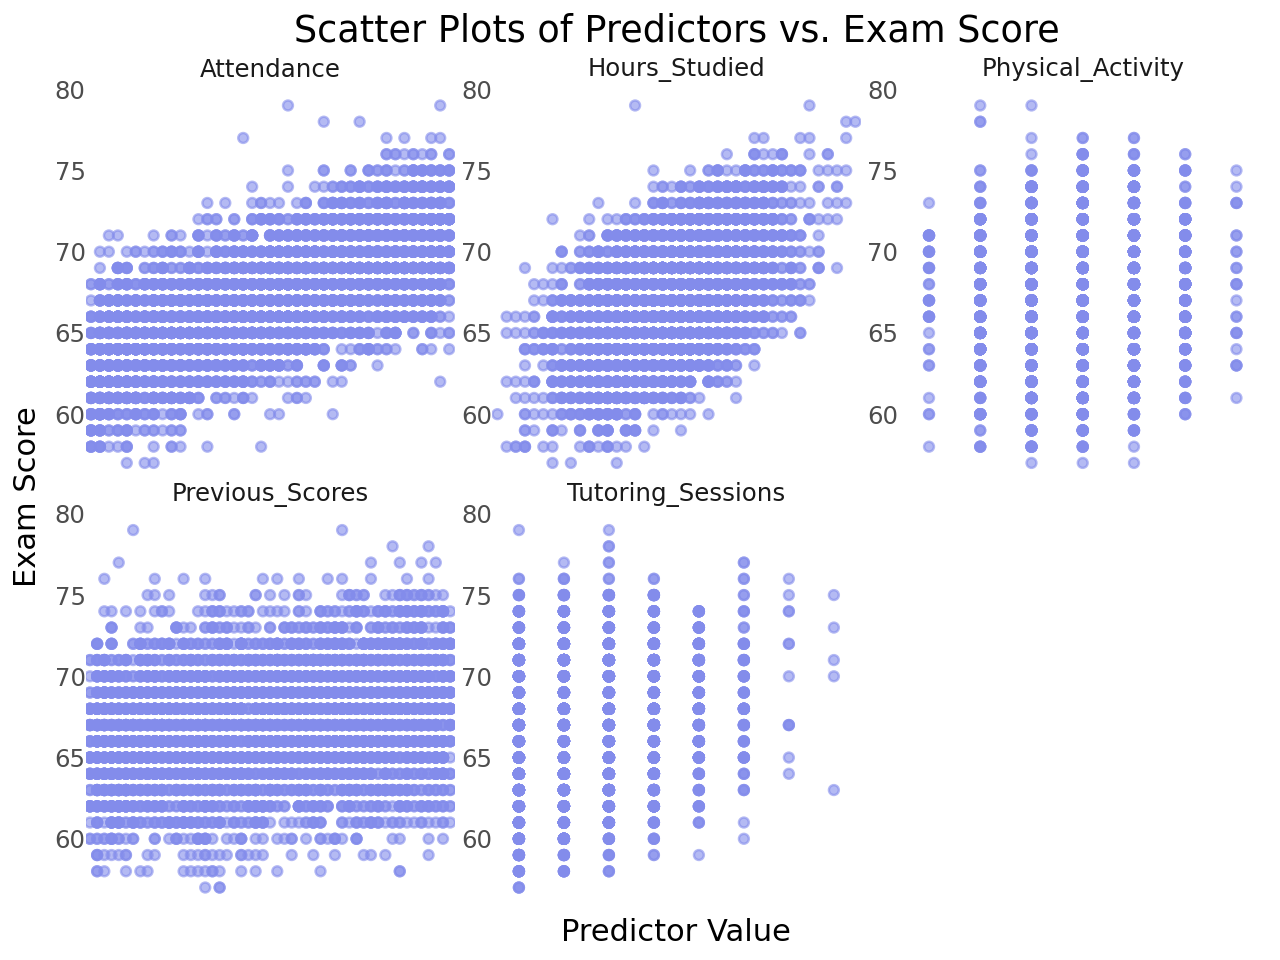
\includegraphics[width=\columnwidth]{10-predictors-vs-exam-score.png}
  \caption{Scatterplot of each predictor vs. Exam Scores for the Low Model}
  \label{10:predictors-scatterplot}
\end{figure*}

\begin{figure*}[h]
  \centering
  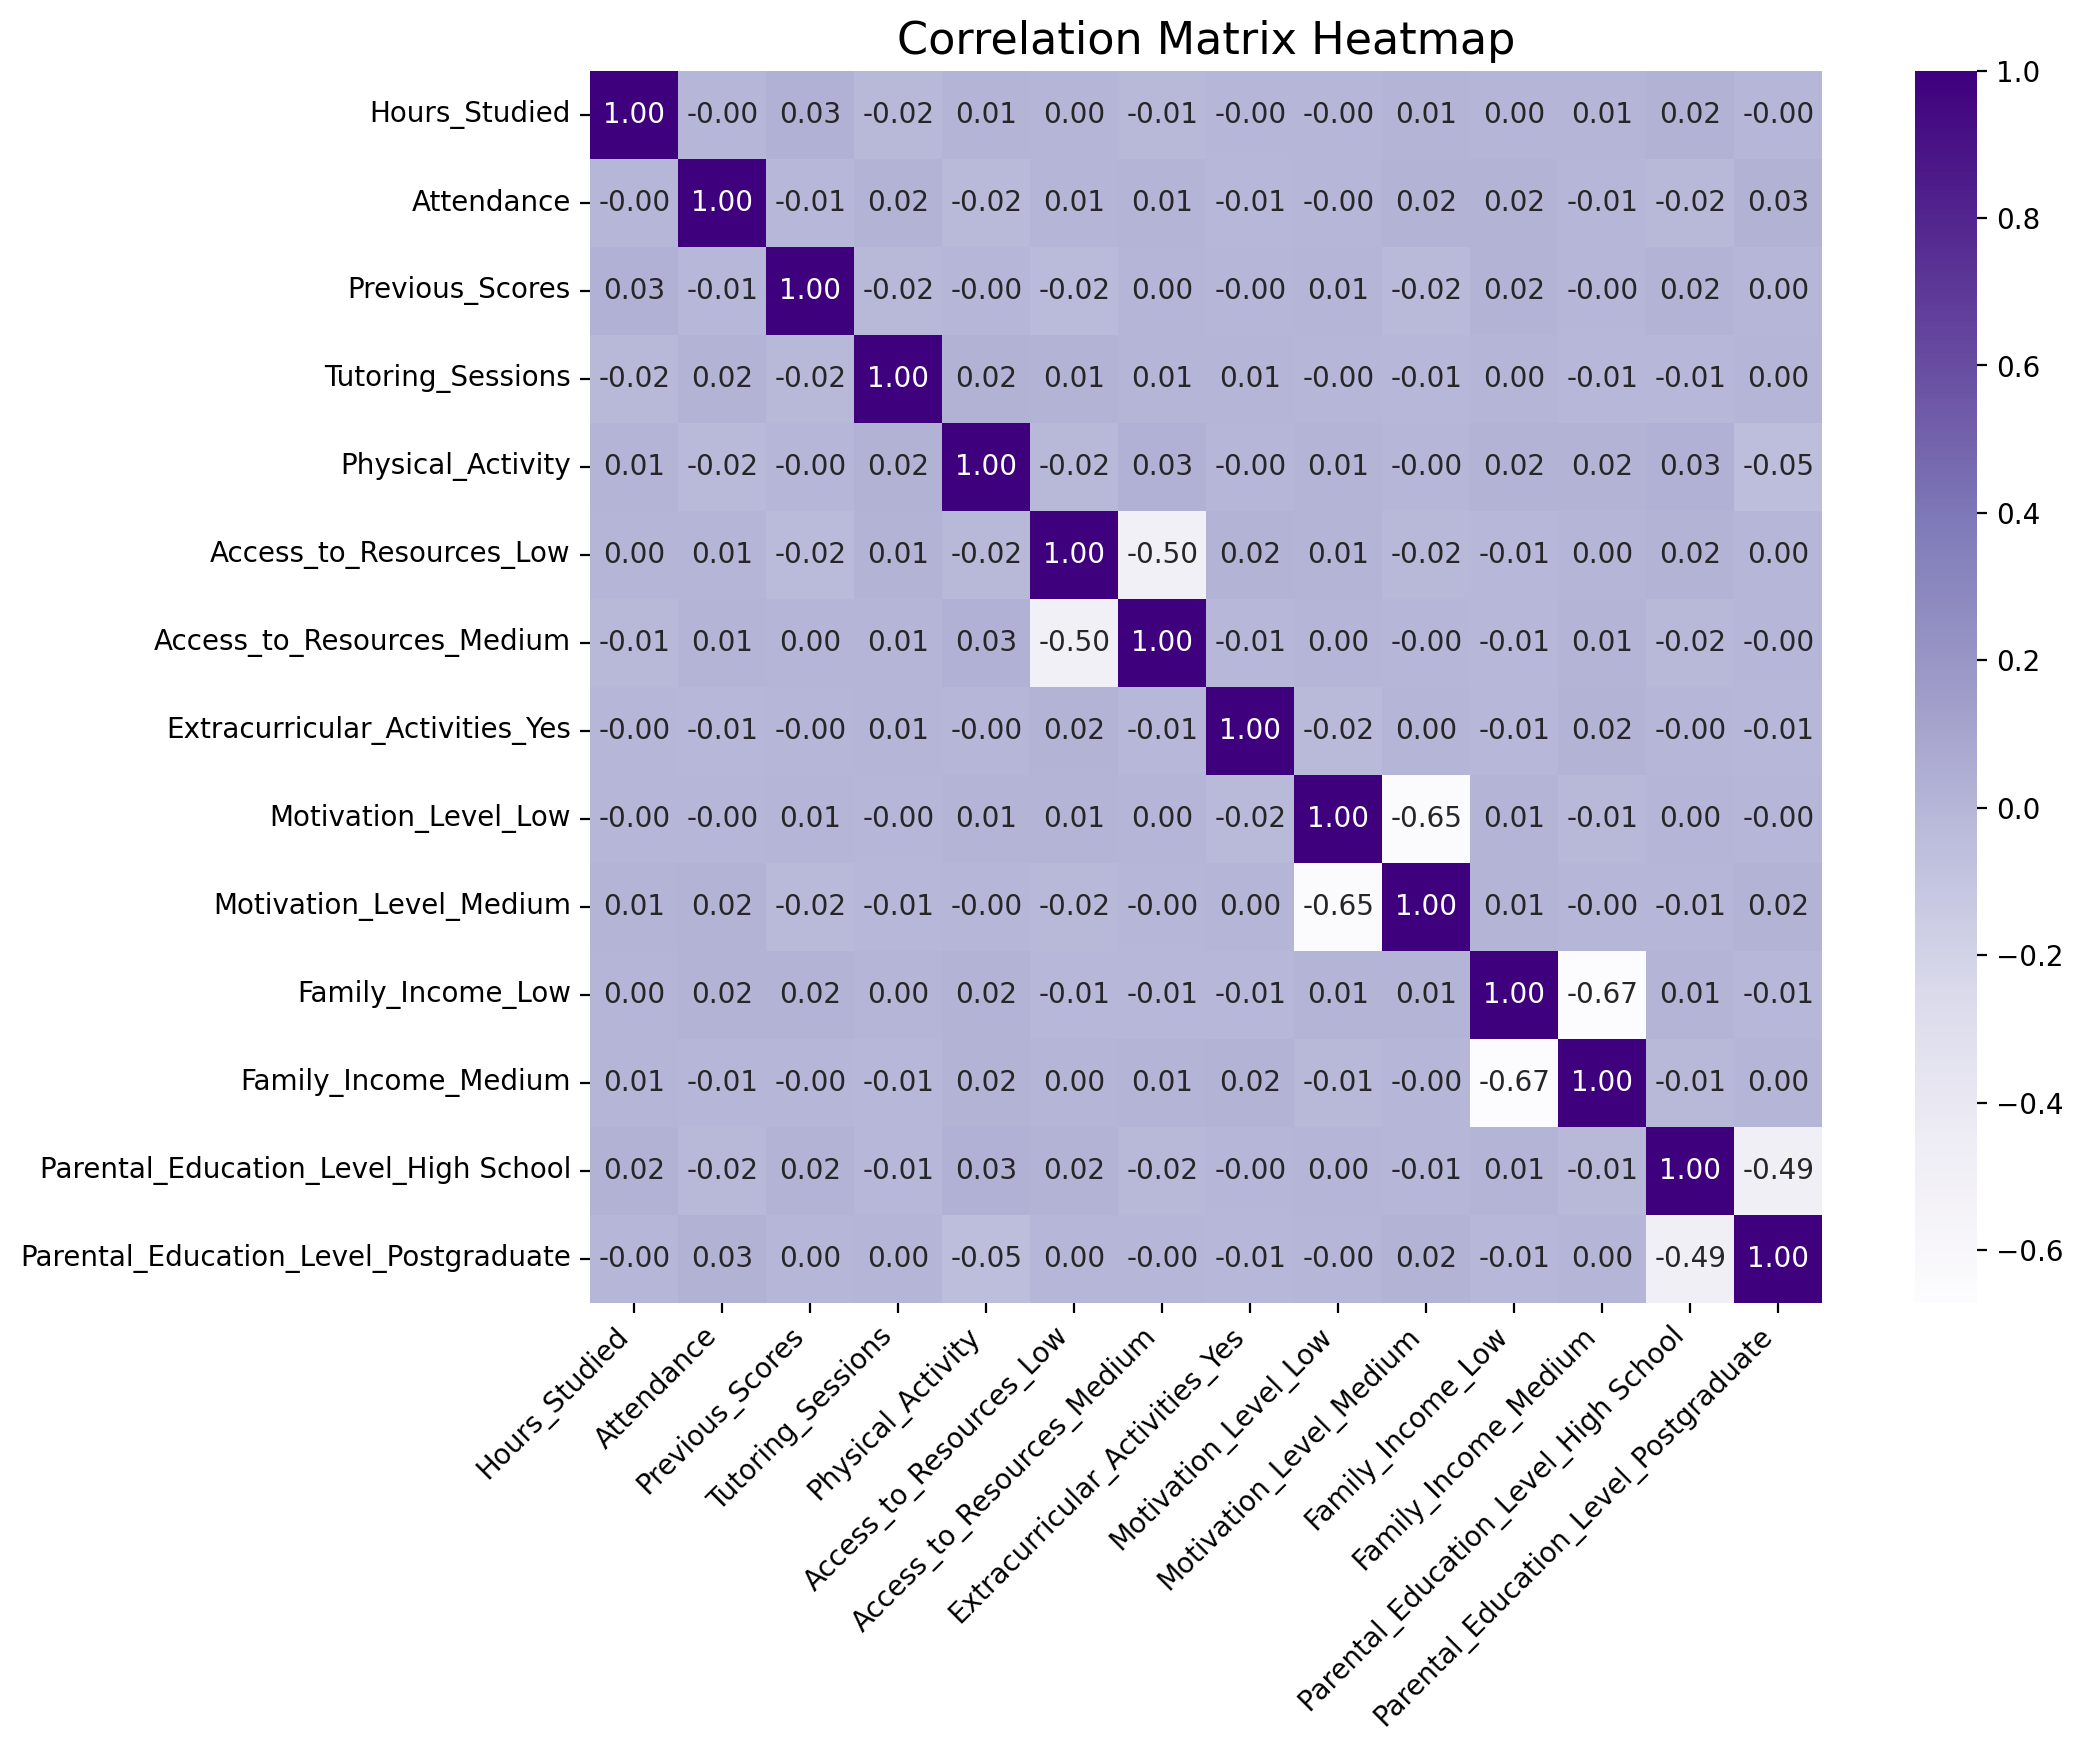
\includegraphics[width=\columnwidth]{11-corr-heatmap.png}
  \caption{Correlation Matrix Heatmap for the Low Model}
  \label{11:corr-heatmap}
\end{figure*}

\begin{figure*}[ht]
  \centering
  
  % First Table
  \begin{subtable}{\textwidth}
    \centering
    \begin{tabular}{lclc}
      \toprule
      \textbf{Dep. Variable:}                             &   Exam\_Score    & \textbf{  R-squared:         } &     0.817   \\
      \textbf{Model:}                                     &       OLS        & \textbf{  Adj. R-squared:    } &     0.677   \\
      \textbf{Method:}                                    &  Least Squares   & \textbf{  F-statistic:       } &     5.845   \\
      \textbf{Date:}                                      & Sat, 12 Oct 2024 & \textbf{  Prob (F-statistic):} &  0.000128   \\
      \textbf{Time:}                                      &     22:38:58     & \textbf{  Log-Likelihood:    } &   -93.933   \\
      \textbf{No. Observations:}                          &          38      & \textbf{  AIC:               } &     221.9   \\
      \textbf{Df Residuals:}                              &          21      & \textbf{  BIC:               } &     249.7   \\
      \textbf{Df Model:}                                  &          16      & \textbf{                     } &             \\
      \textbf{Covariance Type:}                           &    nonrobust     & \textbf{                     } &             \\
      \bottomrule
      \end{tabular}
    \caption{Model Summary Statistics}
    \label{tab:model_summary-high}
  \end{subtable}

  \vspace{1em} % Space between tables
  
  % Second Table
  \begin{subtable}{\textwidth}
    \centering
    \begin{tabular}{lcccccc}
      & \textbf{coef} & \textbf{std err} & \textbf{t} & \textbf{P$> |$t$|$} & \textbf{[0.025} & \textbf{0.975]}  \\
      \midrule
      \textbf{Intercept}                                  &      61.3570  &        8.689     &     7.061  &         0.000        &       43.287    &       79.427     \\
      \textbf{Access\_to\_Resources[T.Low]}               &      -5.7833  &        2.147     &    -2.693  &         0.014        &      -10.249    &       -1.318     \\
      \textbf{Access\_to\_Resources[T.Medium]}            &       0.9025  &        2.073     &     0.435  &         0.668        &       -3.408    &        5.213     \\
      \textbf{Internet\_Access[T.Yes]}                    &       2.4094  &        2.284     &     1.055  &         0.303        &       -2.340    &        7.159     \\
      \textbf{Family\_Income[T.Low]}                      &      -1.2200  &        2.065     &    -0.591  &         0.561        &       -5.514    &        3.074     \\
      \textbf{Family\_Income[T.Medium]}                   &       1.2700  &        1.937     &     0.656  &         0.519        &       -2.758    &        5.298     \\
      \textbf{Teacher\_Quality[T.Low]}                    &      -3.5358  &        3.013     &    -1.174  &         0.254        &       -9.802    &        2.730     \\
      \textbf{Teacher\_Quality[T.Medium]}                 &      -0.6296  &        1.633     &    -0.386  &         0.704        &       -4.025    &        2.766     \\
      \textbf{School\_Type[T.Public]}                     &      -1.9864  &        2.269     &    -0.875  &         0.391        &       -6.705    &        2.732     \\
      \textbf{Parental\_Education\_Level[T.High School]}  &       1.7369  &        1.595     &     1.089  &         0.289        &       -1.581    &        5.055     \\
      \textbf{Parental\_Education\_Level[T.Postgraduate]} &       1.9619  &        2.174     &     0.902  &         0.377        &       -2.560    &        6.484     \\
      \textbf{Gender[T.Male]}                             &      -0.6569  &        1.600     &    -0.411  &         0.686        &       -3.984    &        2.671     \\
      \textbf{Hours\_Studied}                             &       0.1755  &        0.168     &     1.046  &         0.307        &       -0.173    &        0.524     \\
      \textbf{Attendance}                                 &       0.2455  &        0.078     &     3.162  &         0.005        &        0.084    &        0.407     \\
      \textbf{Sleep\_Hours}                               &      -0.6946  &        0.477     &    -1.456  &         0.160        &       -1.687    &        0.298     \\
      \textbf{Previous\_Scores}                           &       0.1439  &        0.048     &     3.009  &         0.007        &        0.044    &        0.243     \\
      \textbf{Tutoring\_Sessions}                         &      -0.3698  &        0.636     &    -0.581  &         0.567        &       -1.692    &        0.953     \\
      \bottomrule
    \end{tabular}
    \caption{Regression Coefficients}
    \label{tab:regression_coefficients-high}
  \end{subtable}

  \vspace{1em} % Space between tables

  % Third Table
  \begin{subtable}{\textwidth}
    \centering
    \begin{tabular}{lclc}
      \textbf{Omnibus:}       &  1.452 & \textbf{  Durbin-Watson:     } &    1.866  \\
      \textbf{Prob(Omnibus):} &  0.484 & \textbf{  Jarque-Bera (JB):  } &    1.252  \\
      \textbf{Skew:}          &  0.429 & \textbf{  Prob(JB):          } &    0.535  \\
      \textbf{Kurtosis:}      &  2.765 & \textbf{  Cond. No.          } & 1.60e+03  \\
      \bottomrule
      \end{tabular}
    \caption{Model Diagnostics}
    \label{tab:model_diagnostics-high}
  \end{subtable}

  \caption{Summary of Regression Results for the High Model}
  \label{fig:high-model-summary}
\end{figure*}

\begin{figure*}[h]
  \centering
  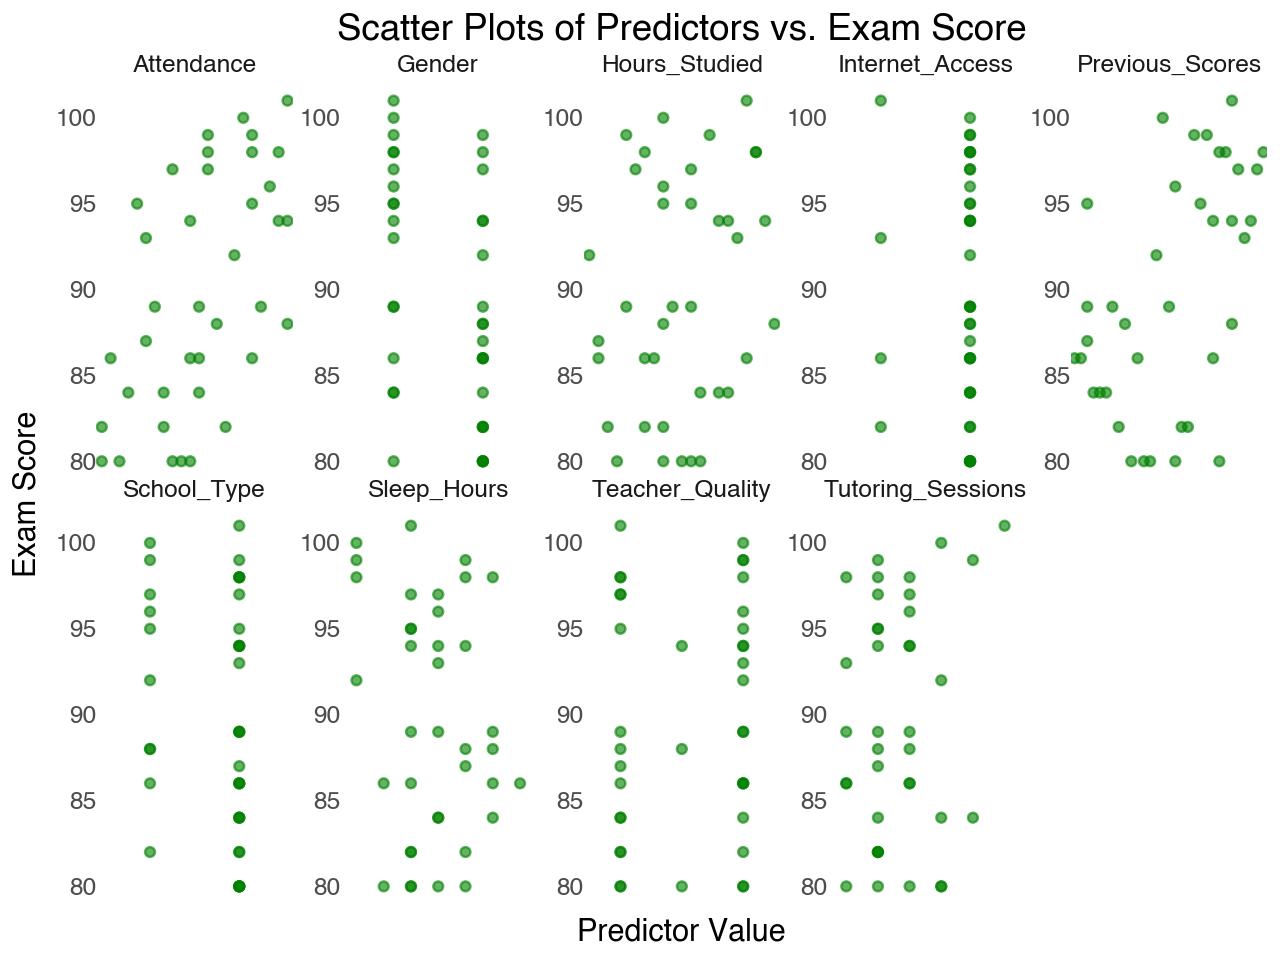
\includegraphics[width=\columnwidth]{20-predictors-scatterplot.png}
  \caption{Scatterplot of each predictor vs. Exam Scores for the High Model}
  \label{20:predictors-scatterplot}
\end{figure*}

\begin{figure*}[h]
  \centering
  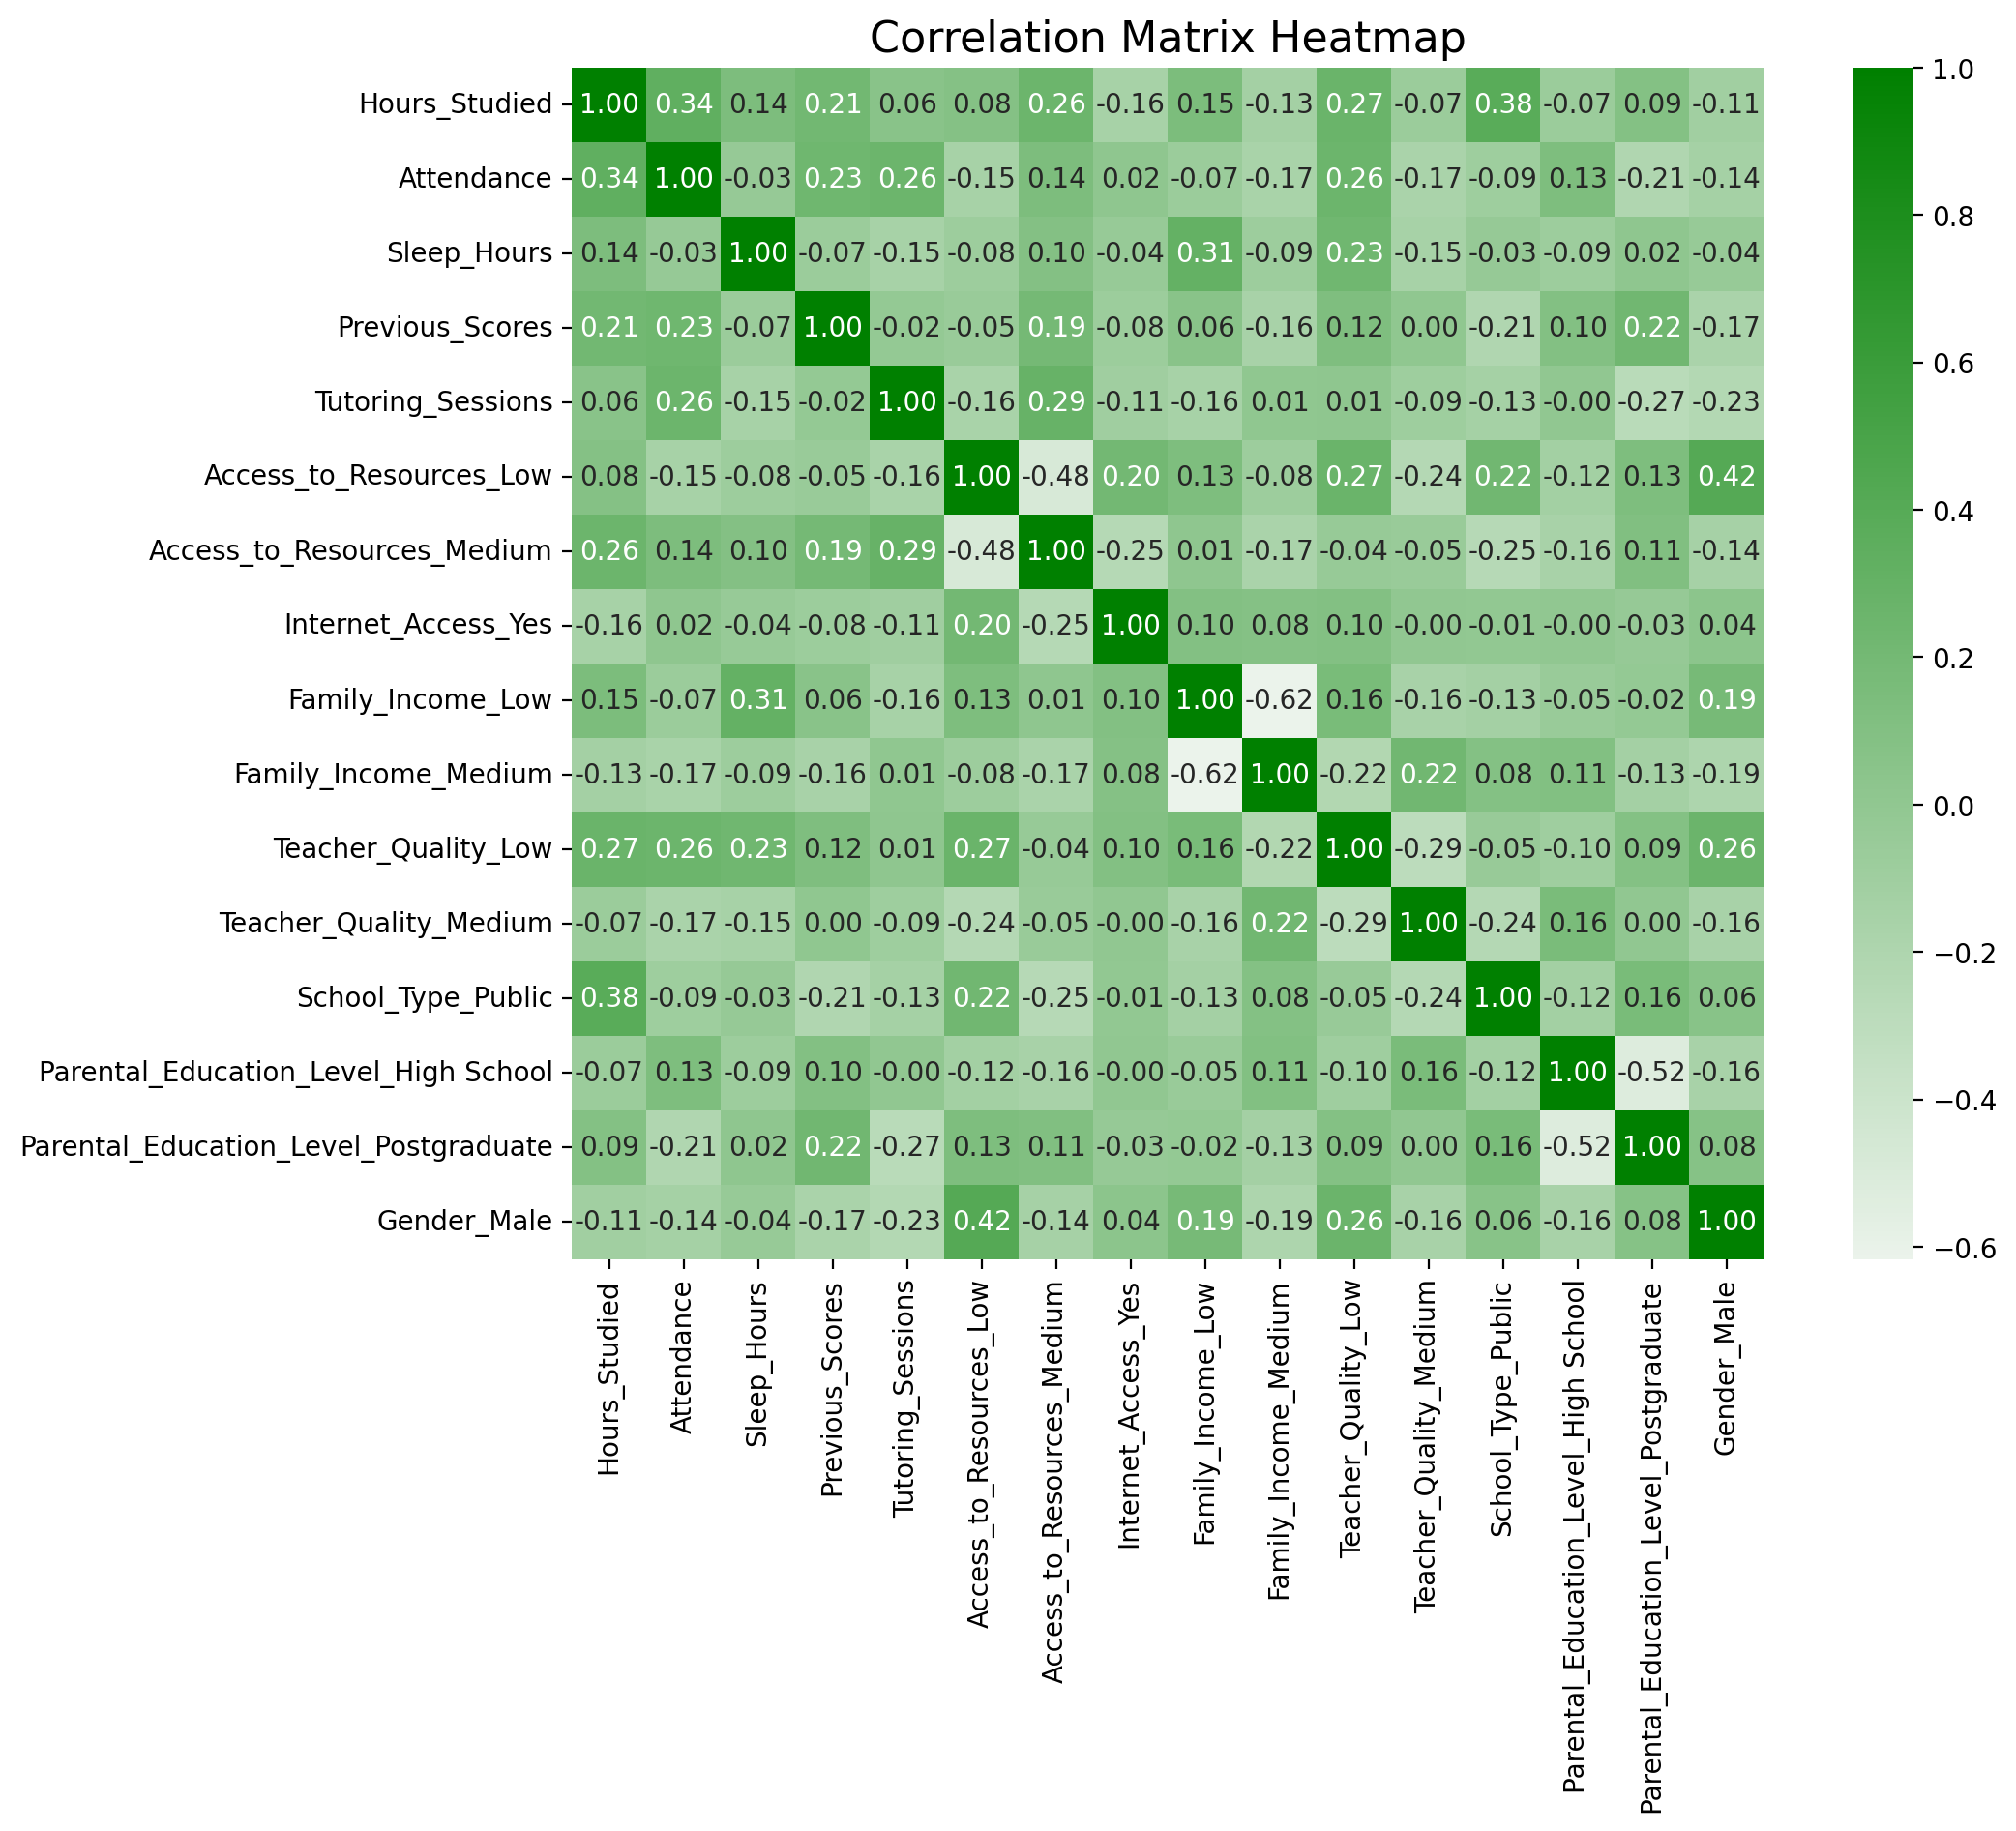
\includegraphics[width=\columnwidth]{21-corr-heatmap.png}
  \caption{Correlation Matrix Heatmap for the High Model}
  \label{21:corr-heatmap}
\end{figure*}

\end{document}
